\documentclass[spanish,a4paper]{beamer}%
%,aspectratio=169

%% CUSTOM COLOR
\definecolor{azuremist}{rgb}{0.94, 1.0, 1.0}
\definecolor{ashgrey}{rgb}{0.7, 0.75, 0.71}
\definecolor{myyellow}{rgb}{.9,.9,.1}
\definecolor{cadmiumorange}{rgb}{0.93, 0.53, 0.18}
\definecolor{carminered}{rgb}{1.0, 0.0, 0.22}
\definecolor{carmine}{rgb}{0.59, 0.0, 0.09}
\definecolor{chromeyellow}{rgb}{1.0, 0.65, 0.0}

%% USE PACKAGE
\usepackage[spanish, es-tabla]{babel}
\usepackage{float}
\usepackage[utf8]{inputenc}
\usepackage{color}
\usepackage{amsmath}
\usepackage{amsfonts}
\usepackage{amssymb}
\usepackage{cite}
\usepackage{epstopdf}
\usepackage{array}
\usepackage{multirow}
\usepackage{multicol}
\usepackage{hyperref}
\usepackage{nameref}
\usepackage{graphicx}
\usepackage{rotating}
\usepackage{enumerate}
\usepackage[font={tiny,color=ashgrey},skip=0pt]{caption}
\usepackage[font={tiny,color=ashgrey},skip=0pt]{subcaption}
\usepackage{changepage}
\usepackage{tikz}
%\usepackage[ backend=biber,style=authortitle,]{biblatex}

\usetheme{Berlin}%Berlin}Luebeck
\usecolortheme[named=chromeyellow]{structure}
%\usecolortheme{lily}

\sloppy
\epstopdfsetup{outdir=./pdf}

%%% NEW COMMANDS
\makeatletter
\let\beamer@writeslidentry@miniframeson=\beamer@writeslidentry%
\def\beamer@writeslidentry@miniframesoff{%
  \expandafter\beamer@ifempty\expandafter{\beamer@framestartpage}{}% does not happen normally
  {%else
    % removed \addtocontents commands
    \clearpage\beamer@notesactions%
  }
}
\newcommand*{\miniframeson}{\let\beamer@writeslidentry=\beamer@writeslidentry@miniframeson}
\newcommand*{\miniframesoff}{\let\beamer@writeslidentry=\beamer@writeslidentry@miniframesoff}
\newcommand\Wider[2][3em]{%
\makebox[\linewidth][c]{%
  \begin{minipage}{\dimexpr\textwidth+#1\relax}
  \raggedright#2
  \end{minipage}%
  }%
}
\setbeamertemplate{headline}
{%
  \begin{beamercolorbox}[colsep=1.5pt]{upper separation line head}
  \end{beamercolorbox}
  \begin{beamercolorbox}{section in head/foot}
    \vskip2pt\insertsectionnavigationhorizontal{\paperwidth}{}{}\vskip2pt
  \end{beamercolorbox}%
  \ifbeamer@theme@subsection%
    \begin{beamercolorbox}[colsep=1.5pt]{middle separation line head}
    \end{beamercolorbox}
    \begin{beamercolorbox}[ht=2.5ex,dp=1.125ex,%
      leftskip=.3cm,rightskip=.3cm plus1fil]{subsection in head/foot}
      \usebeamerfont{subsection in head/foot}\insertsubsectionhead
    \end{beamercolorbox}%
  \fi%
  \begin{beamercolorbox}[colsep=1.5pt]{lower separation line head}
  \end{beamercolorbox}
}
\makeatother
\setbeamerfont{block body}{size=\small}

\makeatletter
	\newcommand*{\currentname}{\@currentlabelname}
	\newcommand{\resCondPath}{\graphicspath{{./figuras/Resultados/conduccion/}}}
	\newcommand{\resRadPath}{\graphicspath{{./figuras/Resultados/radiacion/}}}
	\newcommand{\resDiffMatEspPath}{\graphicspath{{./figuras/Resultados/DiffMatEsp/} }}
	\newcommand{\resRelPath}{\graphicspath{{./figuras/Resultados/RelacionCondRad/}}}
	\newcommand{\generalPath}{\graphicspath{{./figuras/}}}
	\newcommand{\proPath}{\graphicspath{{./figuras/Procedimiento_Simulaciones/}}}
\makeatother

%\usepackage{etoc}
%para generar índice con hipervínculos



%parametros del documento (sus propiedades)
\hypersetup{
    pdftitle={Martin Augusto Reigadas Teran - TFG - 2022},
    pdfsubject={TFG - 2022},
    pdfauthor={Martin Augusto Reigadas Teran},
    pdfkeywords={termo-fotovoltaica} {campo cercano} {recuperación de calor},
    colorlinks,
    citecolor=ashgrey,
    filecolor=ashgrey,
    linkcolor=ashgrey,
    urlcolor=ashgrey,
}

%%%%%%%%%%%%%%%%%%%%%%%%%%%%%%
%%%   TITLE PAGE
\title[\color{white} \tiny Modelado y simulación de espaciadores nanométricos para su aplicación en dispositivos TPVs de campo cercano]{\LARGE Modelado y simulación de espaciadores nanométricos para su aplicación en dispositivos TPVs de campo cercano}
\author[Martin Augusto Reigadas Teran]{\large Martin Augusto Reigadas Teran}
\date{}
\institute{Septiembre, 2022}
\newcommand\InsName{%
  \parbox{.63\textwidth}{%
  \footnotesize\centering Universidad Politécnica de Madrid\\ \vspace{.08cm} Escuela Técnica Superior de Ingeniería y Diseño Industrial\vspace{.1cm} \tiny Grado en Ingeniería Electrónica Industrial y Automática}%
}

\def\Put(#1,#2)#3{\leavevmode\makebox(0,0){\put(#1,#2){#3}}}
 %%% TABLES OF CONTENTS
\AtBeginSection[]
{
\hypersetup{linkcolor=black}
   \begin{frame}<beamer>{\currentname}
        \tableofcontents[currentsection,currentsubsection,hideothersubsections, 
    sectionstyle=show/shaded,subsectionstyle=hide]
   \end{frame}
	\hypersetup{linkcolor=ashgrey}
}
\AtBeginSubsection[]
{
\hypersetup{linkcolor=black}
   \begin{frame}<beamer>{\currentname}
        \tableofcontents[currentsubsection,hideothersubsections, 
    sectionstyle=hide,subsectionstyle=show/shaded/hide]
   \end{frame}
	\hypersetup{linkcolor=ashgrey}
}

%%%%%%%%%%%%%%%%%%%%%%%%%%%%%%%%%%%%%%%%%%%%%%%%%%%%%%%%%%%%%%%%
%%%%%%%%%%%%%%%%%%%%%%%%%%%%%%%%%%%%%%%%%%%%%%%%%%%%%%%%%%%%%%%%
%                        BEGIN DOCUMENT 
%%%%%%%%%%%%%%%%%%%%%%%%%%%%%%%%%%%%%%%%%%%%%%%%%%%%%%%%%%%%%%%%
%%%%%%%%%%%%%%%%%%%%%%%%%%%%%%%%%%%%%%%%%%%%%%%%%%%%%%%%%%%%%%%%
\begin{document}
\generalPath
	%\metroset{block=fill}

	%% TITLE PAGE
	{
		\setbeamercolor{author in head/foot}{use=palette secondary, fg=palette secondary.bg} 
		\setbeamercolor{institute in head/foot}{use=palette secondary, fg=palette secondary.bg}
		\setbeamercolor{section in head/foot}{use=palette tertiary, fg=palette tertiary.bg}
		\setbeamercolor{subsection in head/foot}{use=palette secondary, fg=palette secondary.bg} 
		
		\begingroup
		\setbeamertemplate{headline}{\vspace{0.3cm}%
		\centering
			%\hspace*{0.8cm}%
			%\rule{.15\textwidth}{1.5cm}
			\includegraphics[width=2cm]{figuras/logo_UPM}% \includegraphics for logo 1 goes here
			\raisebox{.6cm}{\InsName}
			%\rule{.15\textwidth}{1.5cm}
			
\includegraphics[width=2.5cm]{figuras/logo_ETSIDI}% \includegraphics for logo 2 goes here
			\hspace*{0.1cm}%
		}
		%%%%%%%%%%%%%%%%%%%%%%%%%%%%%%%%%%%%%%%%%%%%%%%%%%%%%%%%
		%                     TITULO                           %
		%%%%%%%%%%%%%%%%%%%%%%%%%%%%%%%%%%%%%%%%%%%%%%%%%%%%%%%%
		\begin{frame}
		\begin{adjustwidth}{-2em}{-2em}
		\vspace{1cm}
		%
\includegraphics[width=\linewidth,height=.2\textheight]{figuras/cabecera}
		%\vspace{-.2cm}
			%\Put(0,-1cm){\includegraphics[width=2cm]{figuras/logo_UPM}}
			%\Put(0,2cm){}
			\titlepage
			%\begin{titlepage}
				%
\includegraphics[width=\linewidth,height=.1\textheight]{figuras/cabecera.png}
				
				\vspace{-.7cm}
				\begin{minipage}[l]{0.48\textwidth}
				\begin{flushleft}
					\footnotesize \itshape  Tutor: Pablo García-Linares Fontes\\
					\tiny Departamento de Ingeniería Eléctrica, Electrónica, Automática y
			Física Aplicada		
				\end{flushleft}
				\end{minipage}\hfill
				\begin{minipage}[r]{0.48\textwidth}
				\begin{flushright}
					\footnotesize \itshape Cotutora: Esther López Estrada\\
					 \tiny Instituto de Energía Solar\\
					
							
				\end{flushright}
				\end{minipage}
			%\end{titlepage}
			
			\end{adjustwidth}
		\end{frame}
		\endgroup
	}

	%%  TABLA DE CONTENIDOS
	{
		\setbeamercolor{section in head/foot}{use=palette tertiary, fg=palette tertiary.bg}
		\begin{frame}{Tabla de Contenidos}
				\hypersetup{linkcolor=black}
				\tableofcontents[hideallsubsections]
		\end{frame}
	}

	%% INTRODUCCION
	\section{Introducción}
	\begin{frame}{Introducción}
		%%%%%%%%%%%%%%%%%%%%%%%%%%%%%%%%%%%%%%%%%%%%%%%%%%%%%%%
		%           DEMANDA Y CONSUMO DE ENERGÍA   
		%%%%%%%%%%%%%%%%%%%%%%%%%%%%%%%%%%%%%%%%%%%%%%%%%%%%%%
		\vspace{10pt}	
		%% FIGURAS DE DEMANDAS
		\begin{figure}
			\centering
			\begin{subfigure}[b]{0.58\textwidth}
			\centering
				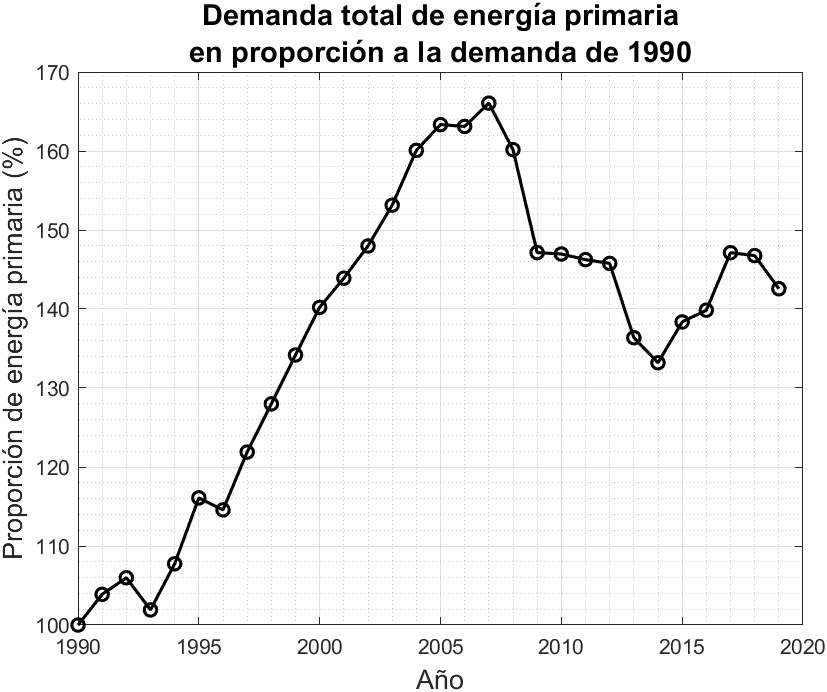
\includegraphics[width=\textwidth]{DemandaEnergiaPrimariaProporcion1990.png}
				\caption*{Fuente de datos: Ministerio para la transición ecológica y el reto demográfico de España.}
			\end{subfigure} \hfill
			\begin{subfigure}[b]{0.4\textwidth}
				\centering
				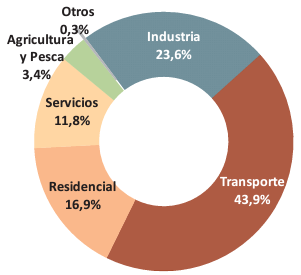
\includegraphics[width=\textwidth]{consumoEnergiaFinalPorSectores_2019.png}
				\caption*{Fuente: Ministerio para la transición ecológica y el reto demográfico de España (2019).}
			\end{subfigure}
			\label{fig:demandaYconsumo}
		\end{figure}
	\end{frame}
	\begin{frame}{Introducción}
		%%%%%%%%%%%%%%%%%%%%%%%%%%%%%%%%%%%%%%%%%%%%%%%%%%%%%%%%%%%%%%%%%%%%%%
		%         MECANISMOS DE GENERACIÓN Y RECUPERACIÓN DE CALOR MECÁNICOS
		%%%%%%%%%%%%%%%%%%%%%%%%%%%%%%%%%%%%%%%%%%%%%%%%%%%%%%%%%%%%%%%%%%%%%%
		\vspace{-10pt}
		%%  FIGURAS SISTEMAS MECANICOS DE GENERACION
		\begin{figure}[htbp]
			\centering
			\onslide<1->{
				\begin{subfigure}[b]{0.55\textwidth}
					\centering
						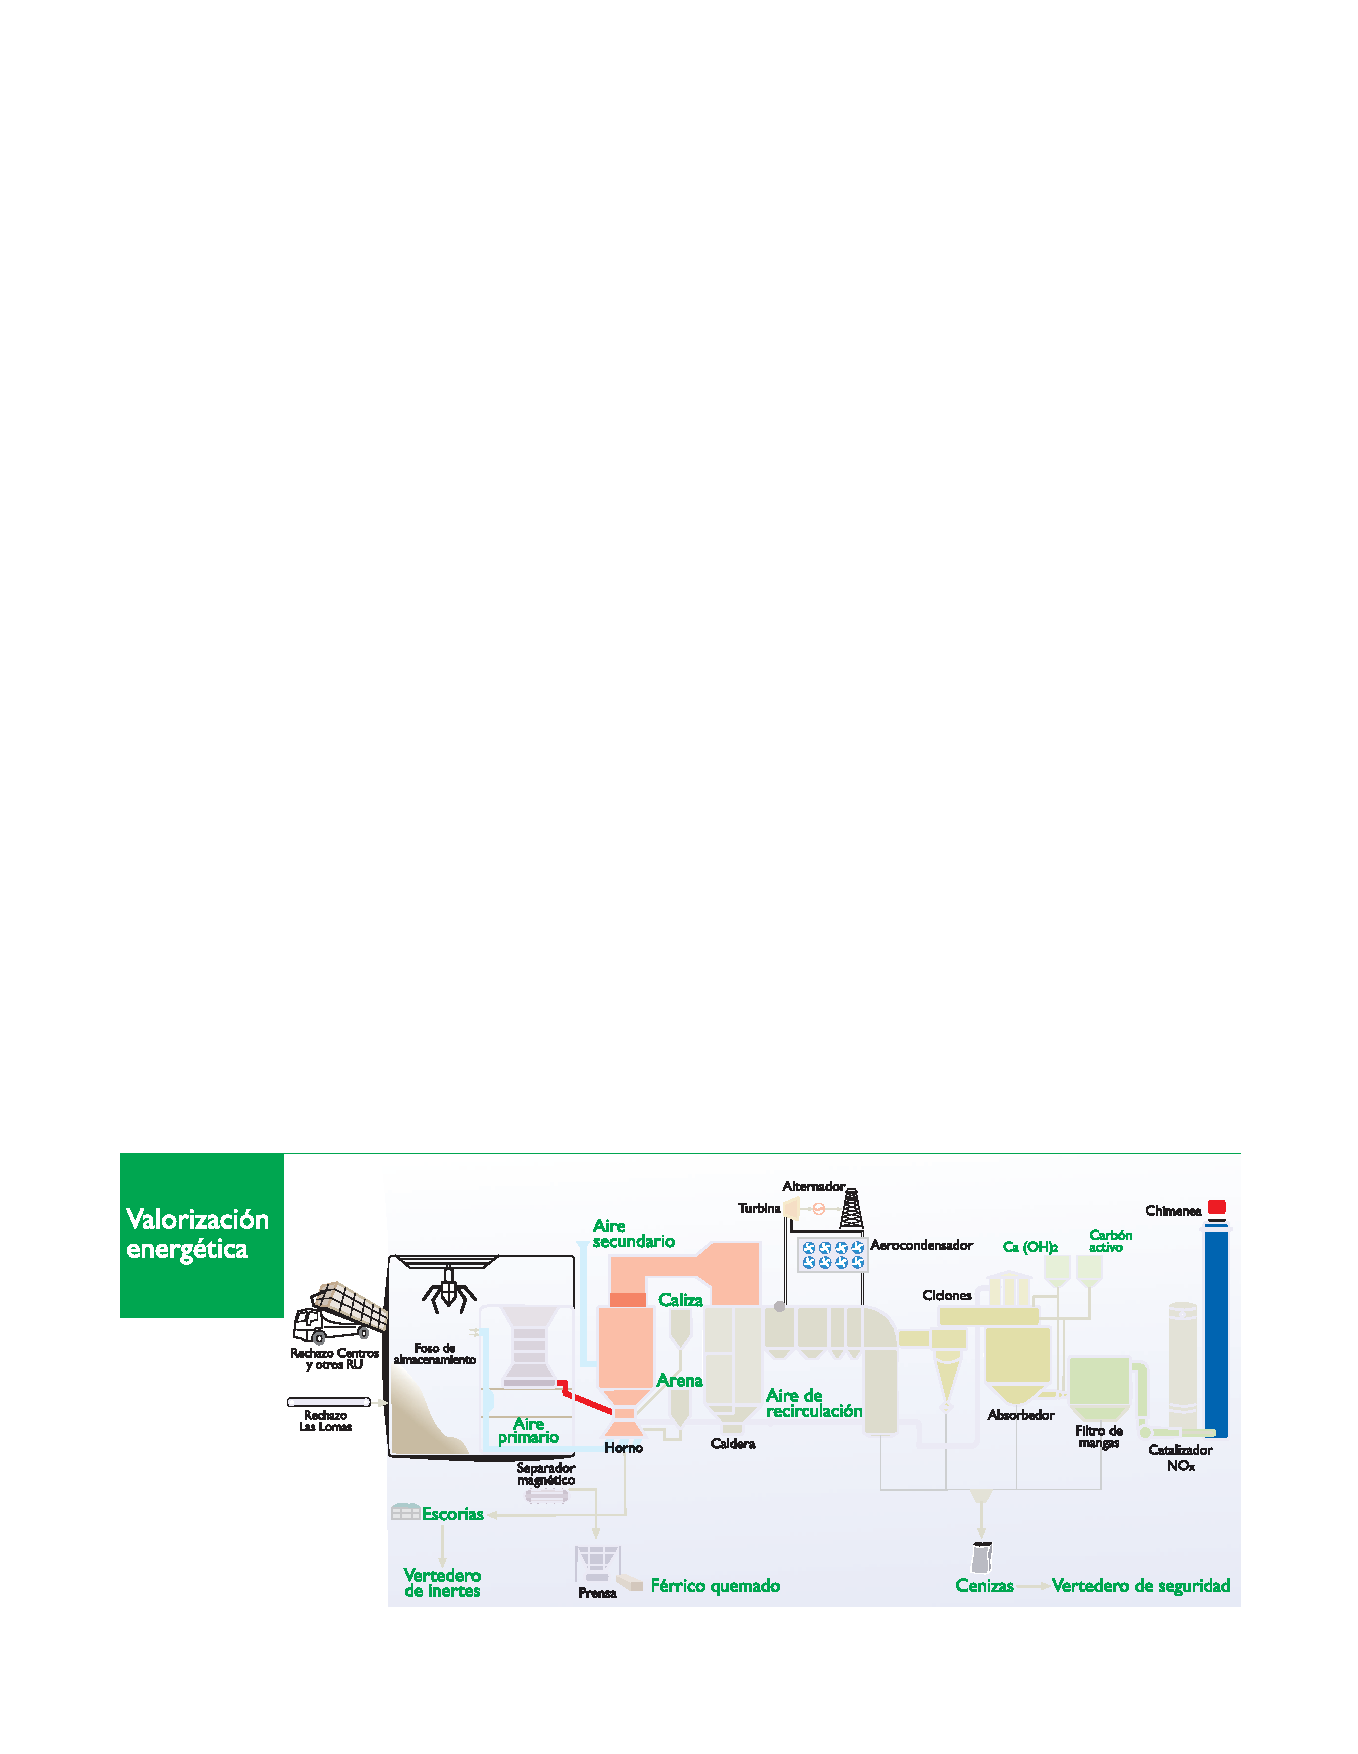
\includegraphics[width=\textwidth]{esquemasLomasValorizacion}
						\caption*{Fuente: Ayuntamiento de Madrid.}
				\end{subfigure}\hfill
			}
			%
			\onslide<2->{
				\begin{subfigure}[b]{0.4\textwidth}
					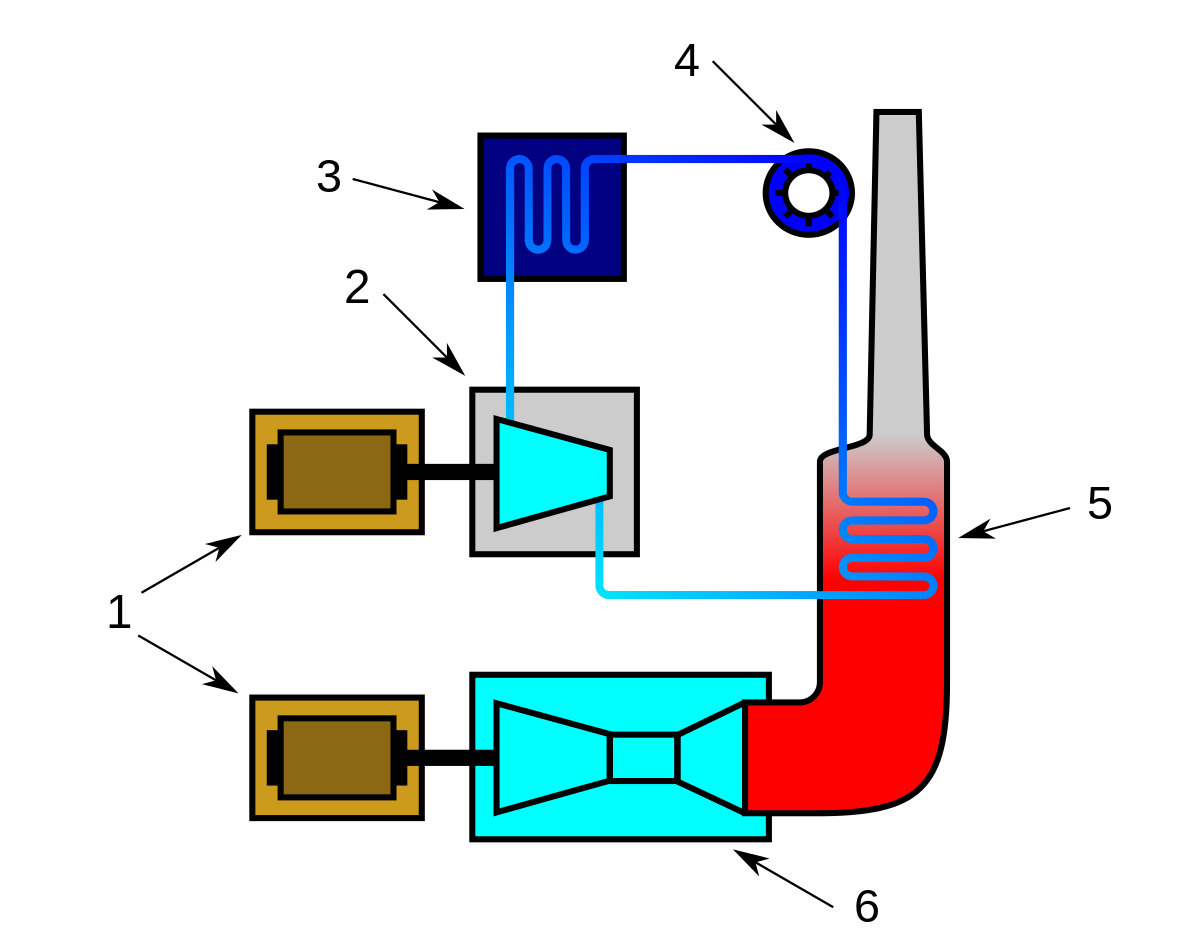
\includegraphics[width=\textwidth]{cicloCombinado}
					\caption*{Ciclo combinado. Fuente: Wikipedia.}
				\end{subfigure} \hfill
			}
			%
			\onslide<3->{
				\begin{subfigure}[b]{0.38\textwidth}
					\vspace{-5pt}
					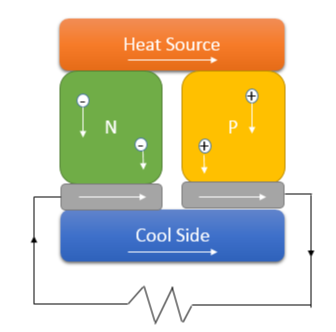
\includegraphics[height=0.4\textheight,width=\textwidth,angle=0]{TEG}
					\caption*{TEG. Fuente: \cite{TEG5efficiency}}
				\end{subfigure}
				\hfill
			}
			\onslide<4>{
				\begin{subfigure}[b]{0.48\textwidth}
					\vspace{-1cm}
					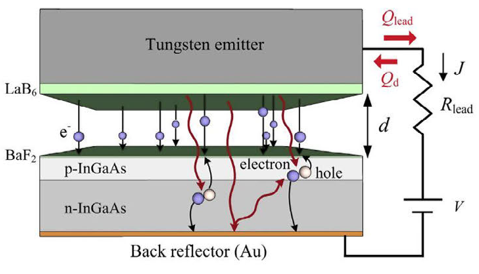
\includegraphics[width=\textwidth]{iTPV}
					\caption*{iTPV. Fuente: \cite{Thermoionic_nTPV_DATAS201910}}
				\end{subfigure} 
			}
			%
			\label{fig:valdemingomez_cc_TEG_iTPV}
		\end{figure}
	\end{frame}
	\begin{frame}{Introducción}
		\begin{figure}[ht]
			\centering
			\onslide<1->{
				%%%%%%%%%%%%%%%%%%%%%%%%%%%%%%%%%%%%%%%%%%%%%%%
				%           	TERMO-FOTOVOLTAICA
				%%%%%%%%%%%%%%%%%%%%%%%%%%%%%%%%%%%%%%%%%%%%%%%
				\hfill
				\begin{subfigure}[b]{0.4\textwidth}
					\centering
						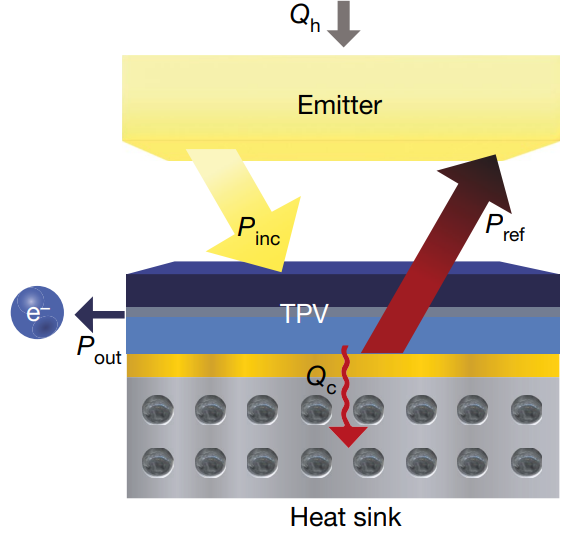
\includegraphics[width=1.00\textwidth]{TPV_40_BSR}
					\caption*{TPV. Fuente: \cite{thermophotovoltaic_40}}
					\label{fig:PV_Effect}
				\end{subfigure}
			}
				%
			\onslide<2->{
				%%%%%%%%%%%%%%%%%%%%%%%%%%%%%%%%%%%%%%%%%%%%%%%%%%%%%%%%
				%                    CAMPO CERCANO
				%%%%%%%%%%%%%%%%%%%%%%%%%%%%%%%%%%%%%%%%%%%%%%%%%%%%%%%%%					
				\hfill
				\begin{subfigure}[b]{0.48\textwidth}
						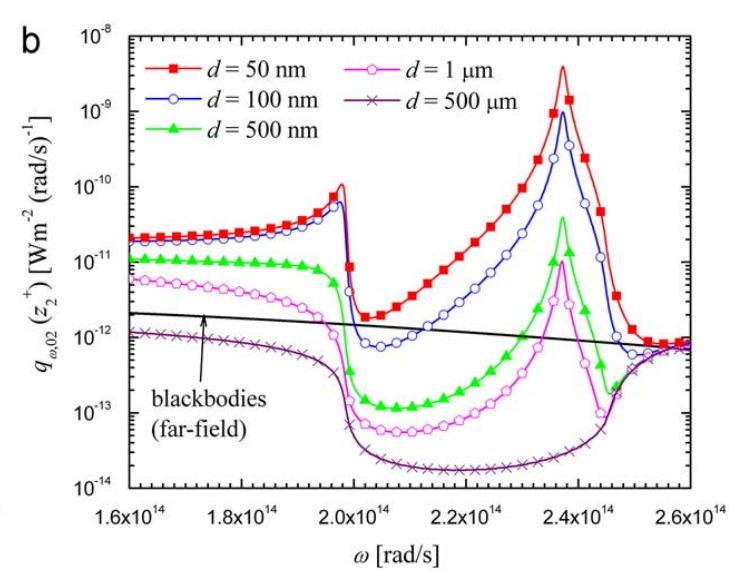
\includegraphics[width=1.00\textwidth]{graficaDiff_dc_fullEqu}
					\caption*{Radiación campo cercano. Fuente: \cite{nfTPV_fullEquations}}
					\label{fig:PV_Effect}
				\end{subfigure}
			}
			\label{fig:TPV}
		\end{figure}
	\end{frame}

%%  CONSIDERACIONES PREVIAS
	\section{Consideraciones previas}
	\begin{frame}{Consideraciones previas}
		\proPath
		\begin{adjustwidth}{-2em}{-2em}
		\begin{figure}\centering	
			\only<2->{
				\begin{subfigure}[c]{.5\textwidth}
					\centering
						
\includegraphics[width=\textwidth]{Conduccion/modelado3D_cerca}
					\label{fig:modelado3D_centro_cerca}
				\end{subfigure}
			}
			\only<4->{
				%\hfill
				\begin{subfigure}[c]{.53\textwidth}
					\centering
						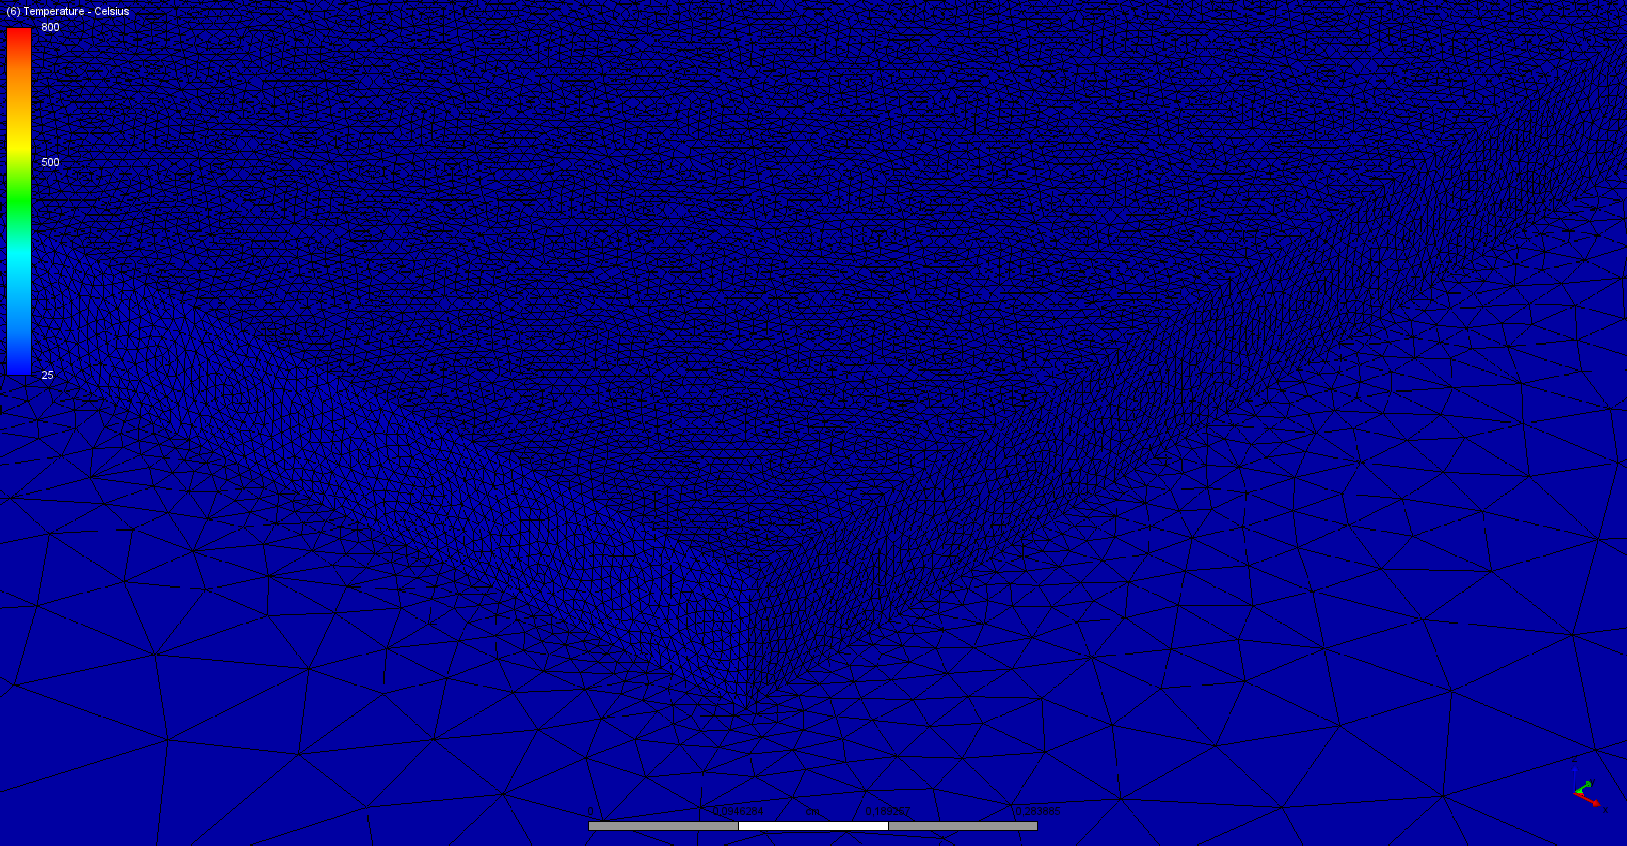
\includegraphics[width=\textwidth]{Conduccion/mallado_100_cerca}
					\label{fig:mallado_100_cerca}
				\end{subfigure}%\hfill
			}
			\only<1->{
				\begin{subfigure}[c]{.4\textwidth}
					\centering
						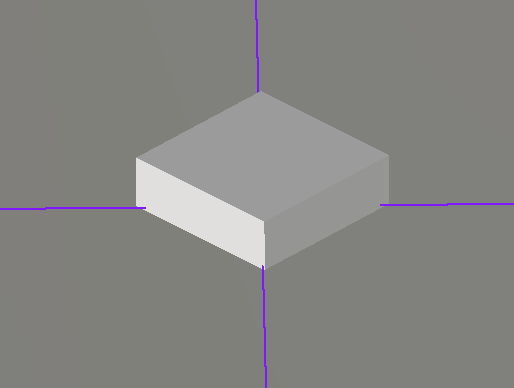
\includegraphics[width=\textwidth]{Conduccion/modelado3D_centro_cerca}
					\label{fig:modelado3D_centro_cerca}
				\end{subfigure}
			}
			\only<3->{
			%\hfill				
				\begin{subfigure}[c]{.67\textwidth}
					\centering
						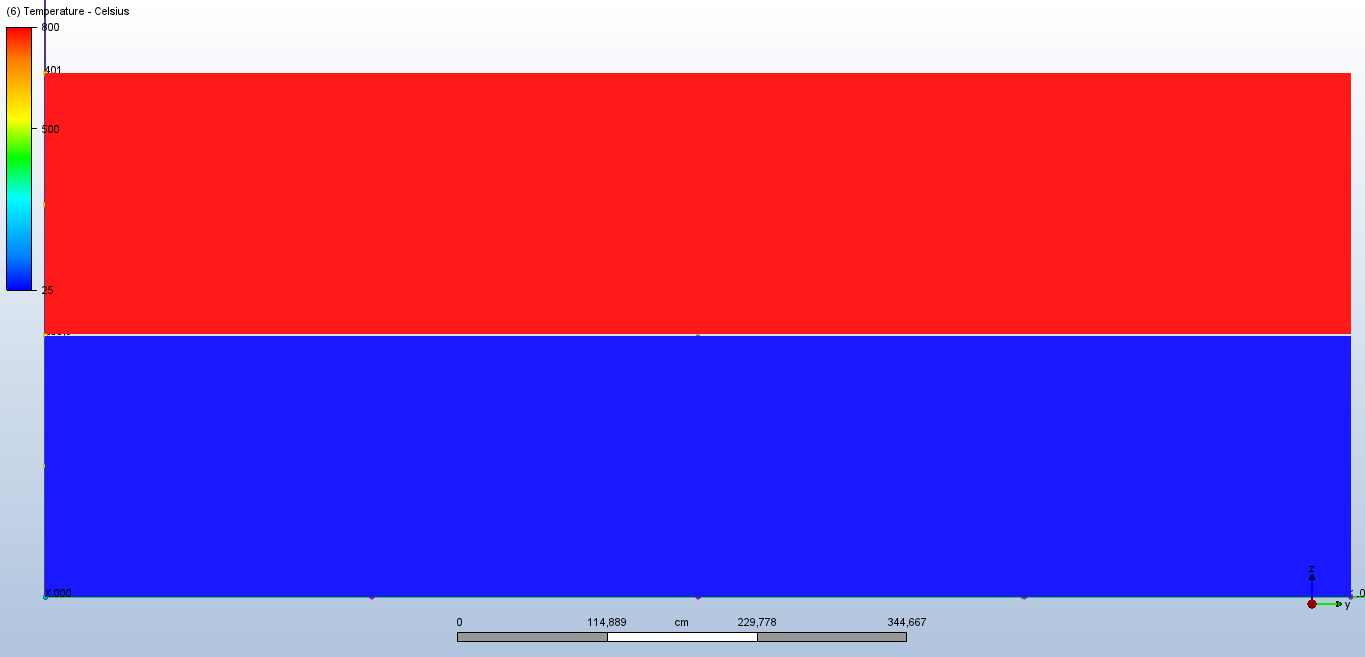
\includegraphics[width=\textwidth]{Conduccion/nTPV_lejos}
					\label{fig:mallado_100_cerca}
				\end{subfigure}
				\vfill	
			}
			\label{fig:CuestionesPrevias}
		\end{figure}
		\end{adjustwidth}
	\end{frame}
	\begin{frame}{Consideraciones previas}
	\proPath
	\begin{adjustwidth}{-2em}{-2em}
		\begin{figure}
			\centering
			\only<1->{
				\begin{subfigure}[c]{.62\textwidth}
					\centering
						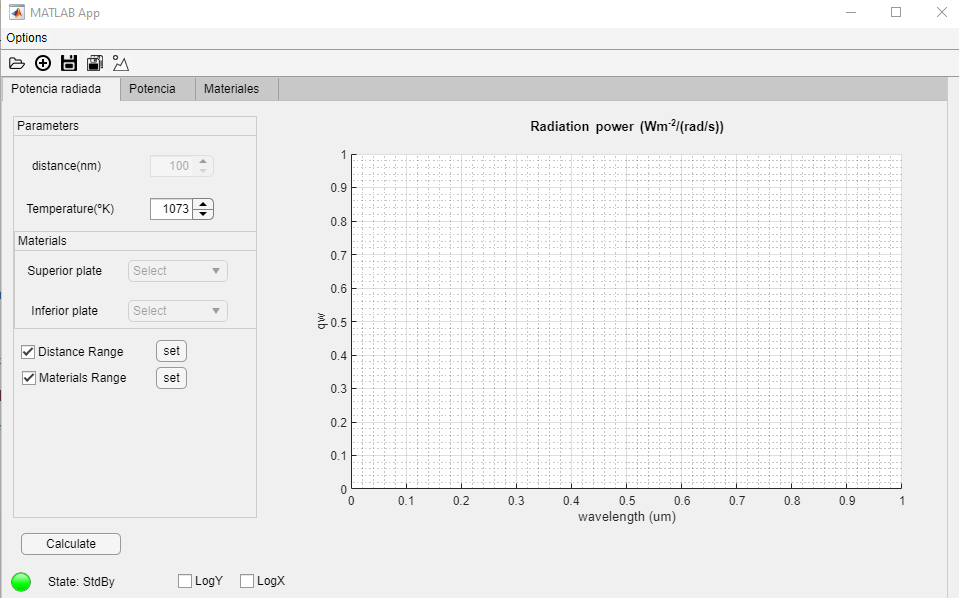
\includegraphics[width=\textwidth]{Radiacion/ejemplo_final_simulacion_radP}
					\label{fig:ejemplo_final_simulacion_radP}
				\end{subfigure}
			}
			\only<2->{
				\begin{subfigure}[c]{.48\textwidth}
					\centering
						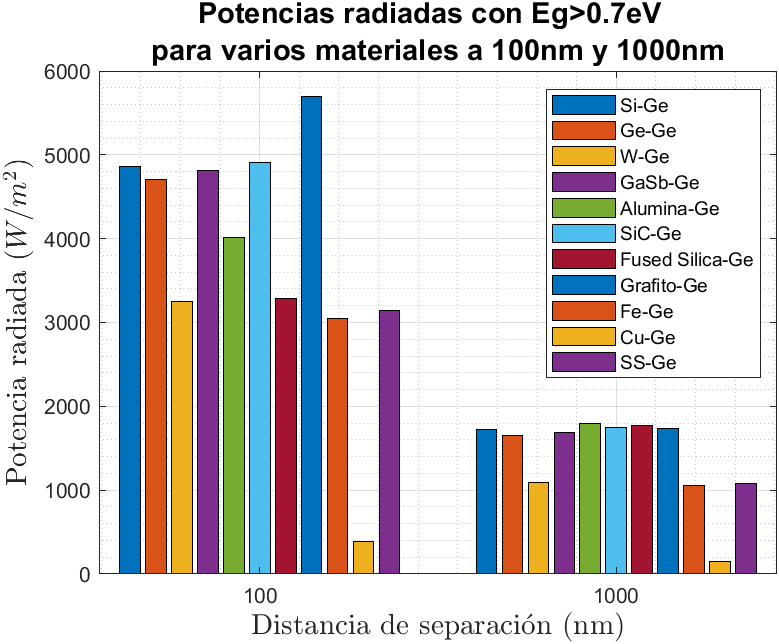
\includegraphics[width=\textwidth]{figuras/rad_mat/EgRad.png}
					\label{fig:EgRad}
				\end{subfigure}
			}
			\label{fig:CuestionesPrevias2}
		\end{figure}
	\end{adjustwidth}
	\end{frame}

%% RESULTADOS
\graphicspath{{./figuras/Resultados}}

	\section{Resultados}
	\begin{frame}{Resultados}
	%\localtableofcontents
	\hypersetup{linkcolor=black}
	%\onehalfspacing
		\tableofcontents[currentsubsection,hideothersubsections, 
    sectionstyle=hide,subsectionstyle=show/show/hide]
		%\hypersetup{linkcolor=ashgrey}
	\end{frame}
	
	\subsection{nTPV Si-SiO2-Si}
	\begin{frame}{nTPV Si-SiO2-Si}
		\only<1>{ %%%   CONDUCCION
			\frametitle{Conducción}
			\resCondPath
			\begin{columns}
			\column{.5\textwidth}
					\vspace{-10pt}
					\begin{block}{\centering Sin Rc}
					\end{block}
					\vspace{-10pt}
					\begin{figure}%
							\centering
							\begin{subfigure}[b]{0.9\columnwidth}
									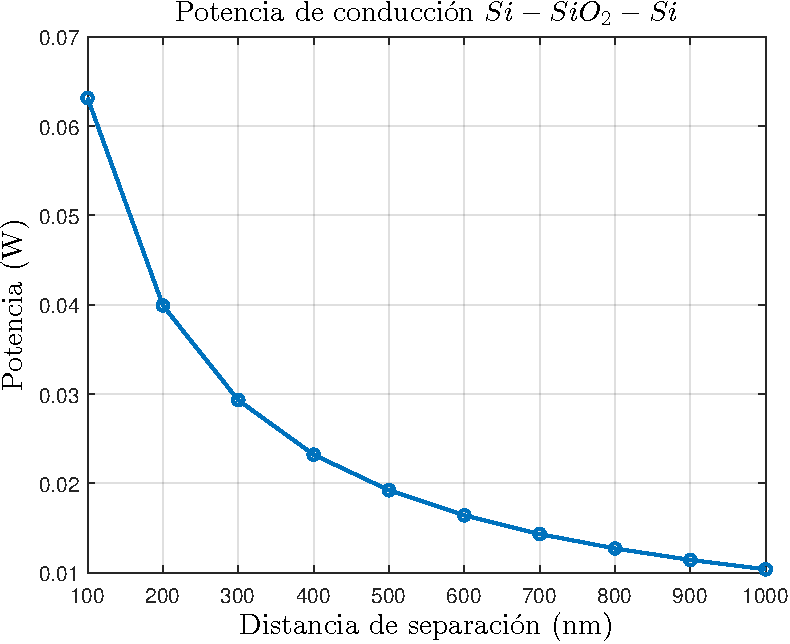
\includegraphics[width=\textwidth]{Pn_SiSiO2Si}
							\end{subfigure}\hfill \vfill
							\begin{subfigure}[b]{0.82\columnwidth}
									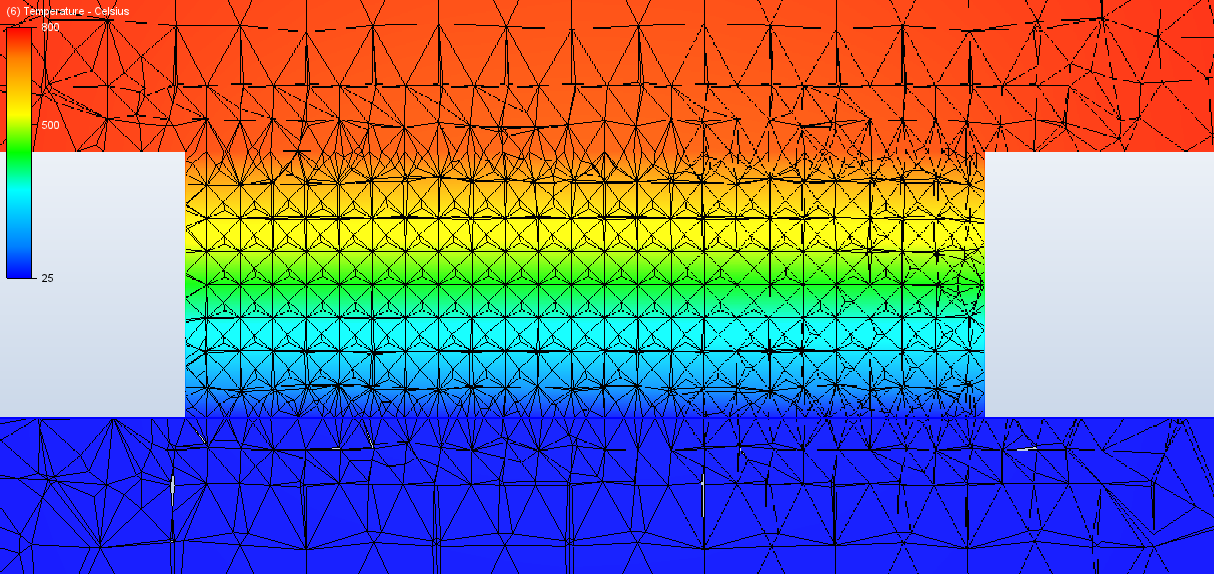
\includegraphics[width=\textwidth]{SiSiO2Si_1000nm_Plane2}%
							\end{subfigure}
							\label{fig:SiSiO2Si_cond}%Pn_SiCSiO2Ge
					\end{figure}
			\column{.5\textwidth}
			\vspace{-10pt}
					\begin{block}{\centering Con Rc}
					\end{block}
			\vspace{-10pt}
			\begin{figure}%
			\centering
			\begin{subfigure}[b]{0.9\columnwidth}
				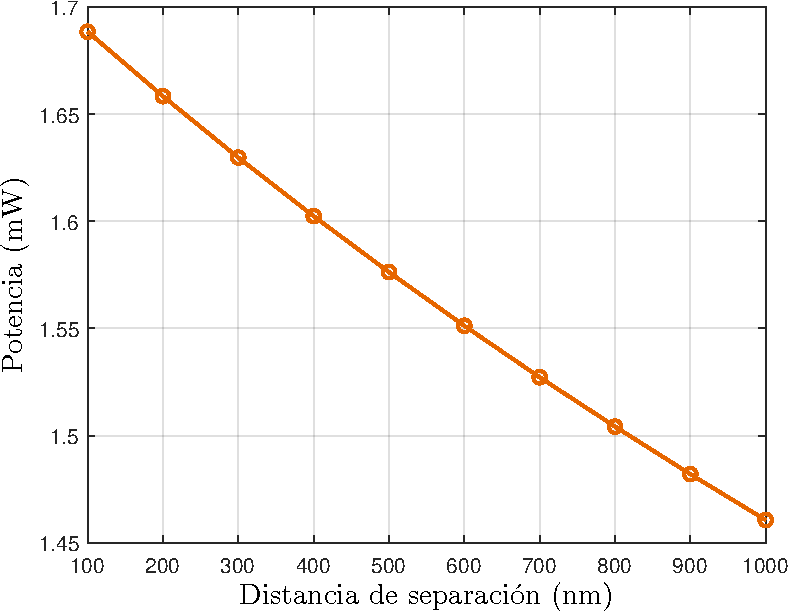
\includegraphics[width=\textwidth]{Prc2_SiSiO2Si}%
			\end{subfigure}
				\hfill \vfill
			\begin{subfigure}[b]{0.8\columnwidth}
				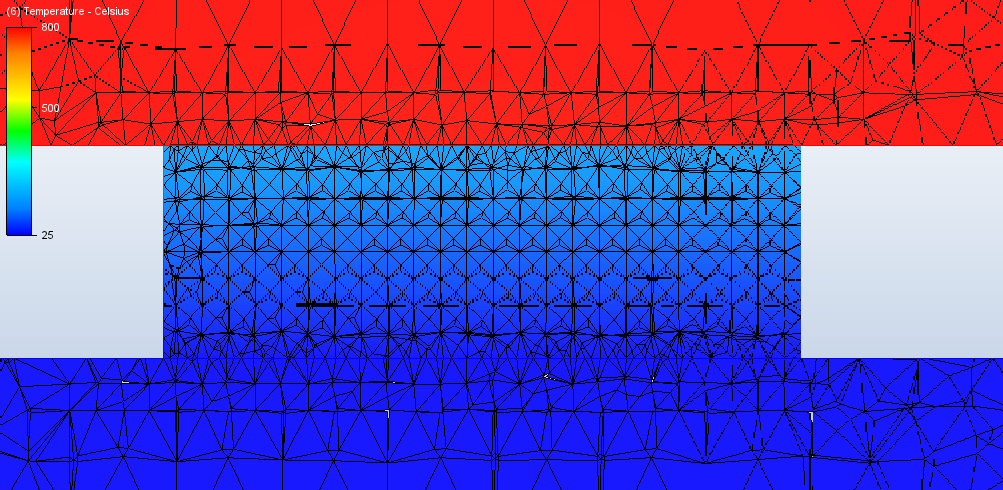
\includegraphics[width=\textwidth]{SiSiO2Si_1000nm_Plane_Rc}
			\end{subfigure}
				\label{fig:SiSiO2Si_condRc}%
			\end{figure}
			\end{columns}			
		}
		\only<2>{
			\frametitle{Conducción: Efectos de la porosidad}
			\resCondPath
			\begin{columns}
			\column{.55\textwidth}
			
			\begin{figure}[t]
				\centering
					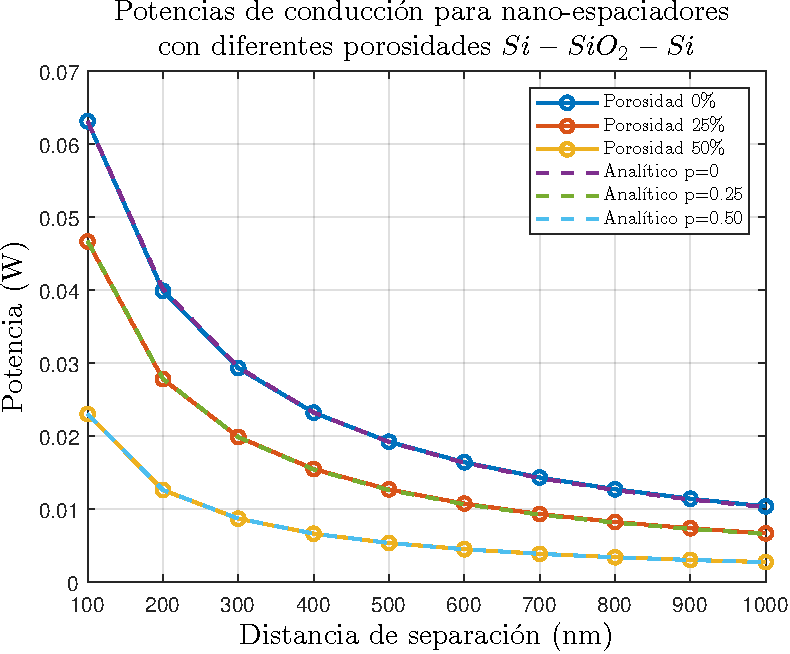
\includegraphics[width=1.00\columnwidth]{Ppor_SiSiO2Si}
				\label{fig:Ppor_SiSiO2Si}
			\end{figure}
			
			\column{.45\textwidth}
			\begin{block}{Módelo analítico}
			 \centering 
				\itshape $P(d,\rho)=- \frac{  16.47\cdot \rho-11.03 }{d-106.80\cdot \rho +74.68}$
			\end{block}
			\end{columns}
		}
		%%%  RADIACION
		\only<3>{
			\frametitle{Radiación}
			\resRadPath
			\begin{columns}
			%%
				\column{.5\textwidth}
					%\vspace{-10pt}
						\begin{block}{\centering Por longitud de onda}
						\end{block}
					\vspace{15pt}
						\begin{figure}[h]%
								\centering
										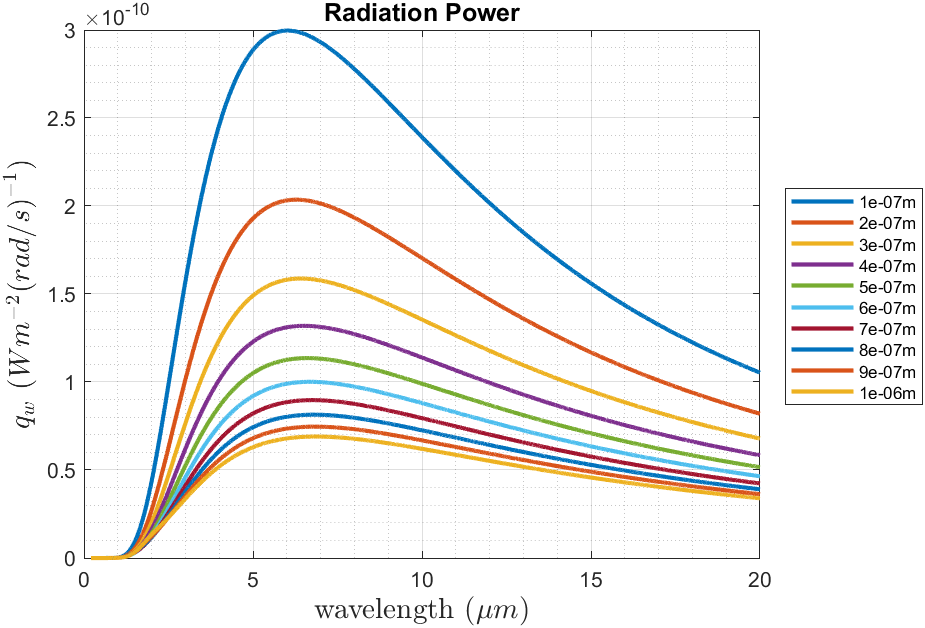
\includegraphics[width=\columnwidth]{SiSi_ds}
								\label{fig:SiSiO2Si_rad}%Pn_SiCSiO2Ge
						\end{figure}
						\vfill
						%%
				\column{.5\textwidth}
					\vspace{-10pt}
						\begin{block}{\centering En el rango de $E>1.1eV$}
							\end{block}
					\vspace{10pt}
						\begin{figure}[h]%
								\centering
										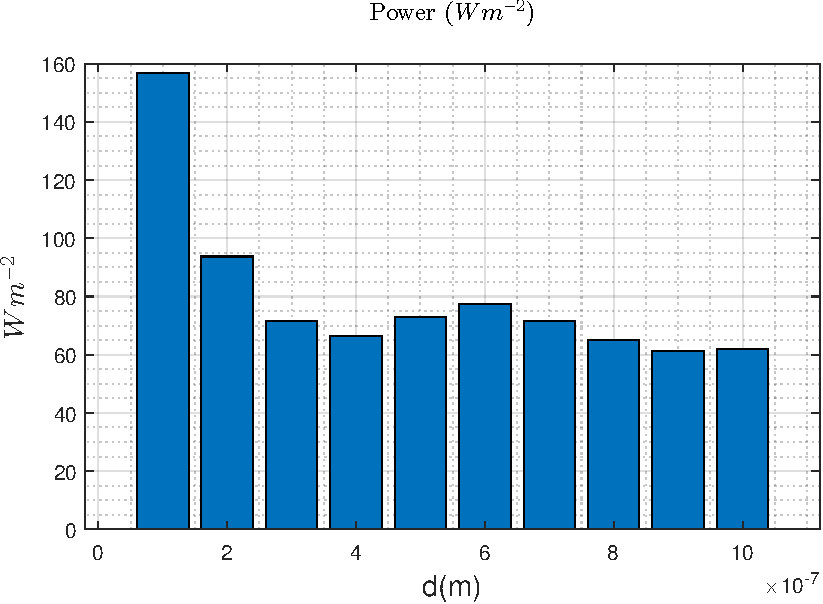
\includegraphics[width=\columnwidth]{p_11_SiSi}%
								\label{fig:SiSiO2Si_radInt}%
						\end{figure}
						\vfill
				\end{columns}		
		}
		%%%  DENSIDADES DE NANO-ESPACIADORES
		\only<4>{
			\frametitle{Densidades de nano-espaciadores ({\small $n^{\circ}esp/cm^2$}) y {\small $E>1.1eV$}}
			\resRelPath
			\begin{columns}
			%%
				\column{.5\textwidth}
					%\vspace{-1cm}
						\begin{block}{\centering Sin Rc}
						\end{block}
					\vspace{10pt}
						\begin{figure}[h]%
								\centering
										\includegraphics[width=\columnwidth]{rel_SiSi11}
								\label{fig:SiSiO2Si_rel}%Pn_SiCSiO2Ge
						\end{figure}
						\vfill
						%%
				\column{.5\textwidth}
					\vspace{-12pt}
						\begin{block}{\centering Con Rc}
							\end{block}
					\vspace{10pt}
						\begin{figure}[h]%
								\centering
										\includegraphics[width=\columnwidth]{rel_SiSi11_Rc}%
								\label{fig:SiSiO2Si_relRc}%
						\end{figure}
						\vfill
				\end{columns}		
		}
	\end{frame}
	
	\subsection{nTPV Si-SiO2-Ge}
	\begin{frame}{nTPV Si-SiO2-Ge}
			\only<1>{ %%%   CONDUCCION
			\frametitle{Conducción}
			\resCondPath
			\begin{columns}
			%%
				\column{.5\textwidth}
					%\vspace{-10pt}
						\begin{block}{\centering Sin Rc}
						\end{block}
					\vspace{15pt}
						\begin{figure}[h]%
								\centering
										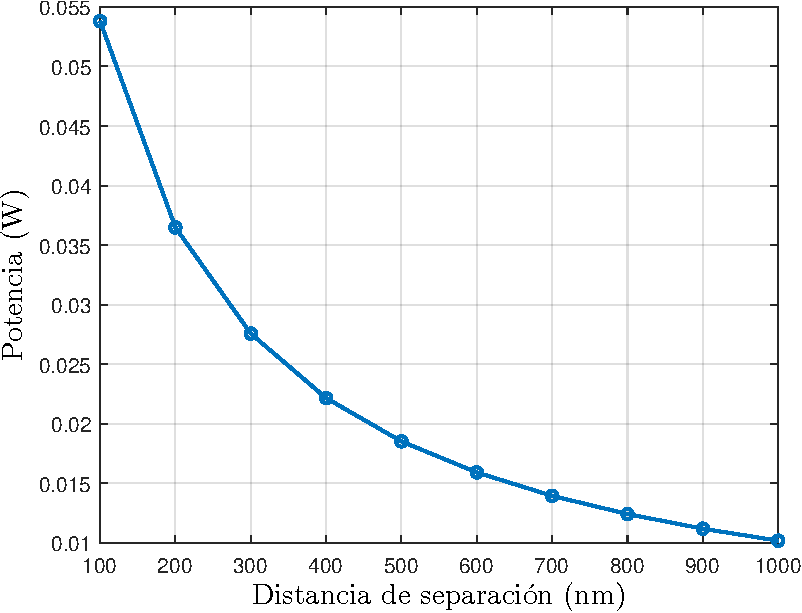
\includegraphics[width=\columnwidth]{Pn_SiSiO2Ge}
								\label{fig:SiSiO2Ge_cond}%Pn_SiCSiO2Ge
						\end{figure}
						\vfill
						%%
				\column{.5\textwidth}
					\vspace{-15pt}
						\begin{block}{\centering En el rango de $E>0.7eV$}
							\end{block}
					\vspace{10pt}
						\begin{figure}[h]%
								\centering
										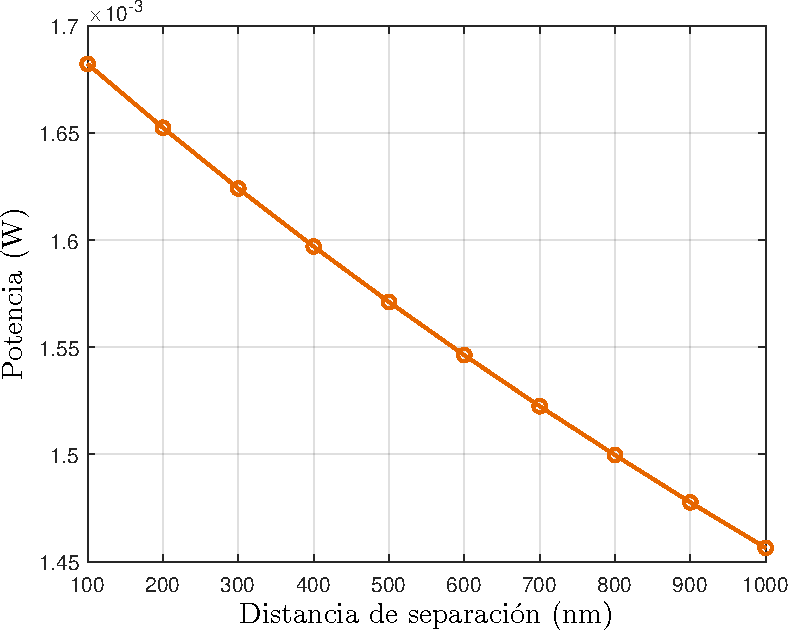
\includegraphics[width=\columnwidth]{Prc2_SiSiO2Ge}%
								\label{fig:SiSiO2Ge_condRc}%
						\end{figure}
						\vfill
				\end{columns}							
		}
		%%%  RADIACION
		\only<2>{
			\frametitle{Radiación}
			\resRadPath
			\begin{columns}
			%%
				\column{.5\textwidth}
					%\vspace{-10pt}
						\begin{block}{\centering Por longitud de onda}
						\end{block}
					\vspace{15pt}
						\begin{figure}[h]%
								\centering
										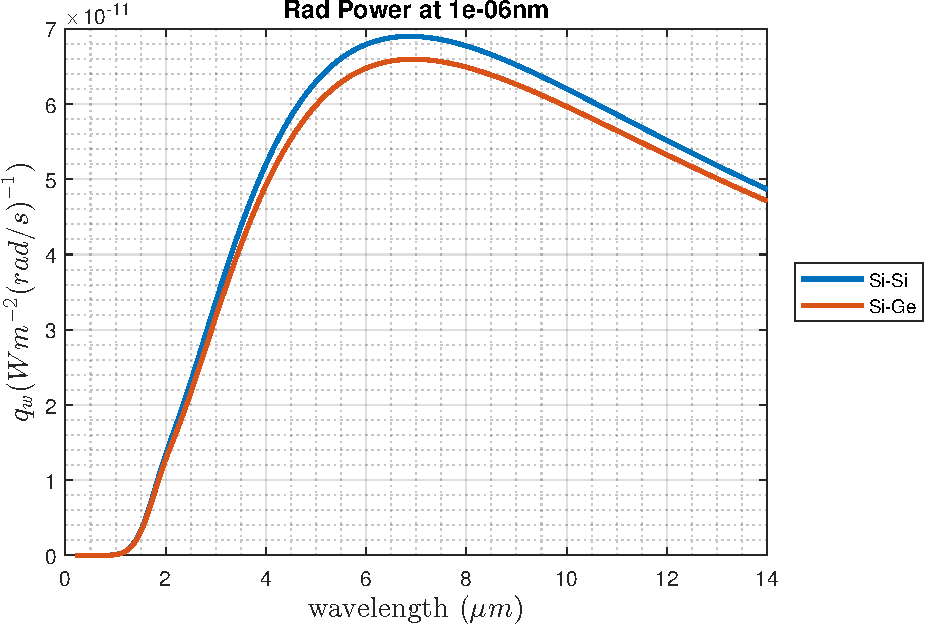
\includegraphics[width=\columnwidth]{SiSi_vs_SiGe}
								\label{fig:SiSivsSiGe_rad}%Pn_SiCSiO2Ge
						\end{figure}
						\vfill
						%%
				\column{.5\textwidth}
					\vspace{-10pt}
						\begin{block}{\centering En el rango de $E>0.7eV$}
							\end{block}
					\vspace{10pt}
						\begin{figure}[h]%
								\centering
										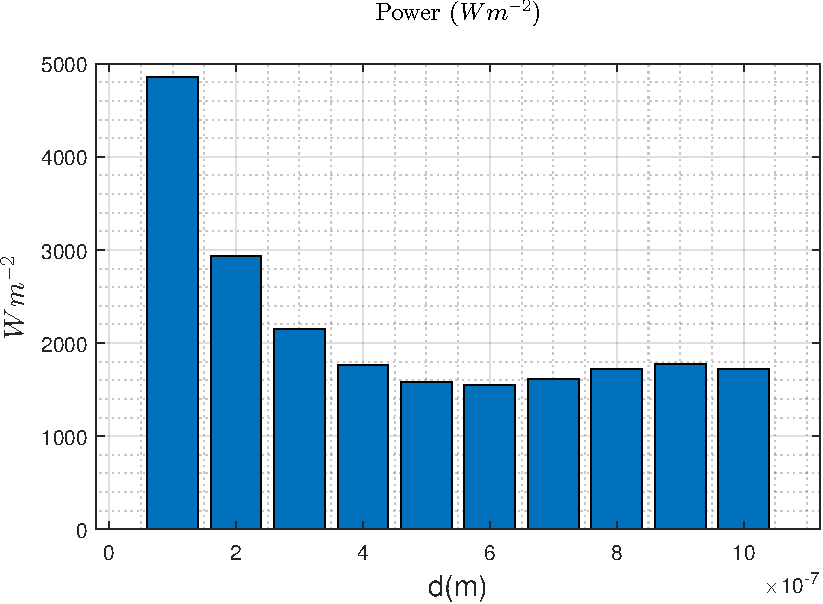
\includegraphics[width=\columnwidth]{p_Eg_SiGe}%
								\label{fig:SiSiO2Ge_radInt}%
						\end{figure}
						\vfill
				\end{columns}		
		}
		%%%  DENSIDADES DE NANO-ESPACIADORES
		\only<3>{
			\frametitle{Densidades de nano-espaciadores ($n^{\circ}esp/cm^2$)}
			\resRelPath
			\begin{columns}
			%%
				\column{.5\textwidth}
					\vspace{-.3cm}
						\begin{block}{\centering Sin Rc}
						\end{block}
					\vspace{0pt}
					\begin{minipage}[l]{.1\columnwidth}
							\begin{turn}{90}
							\begin{minipage}[t]{80pt}
								\begin{block}{\centering Rango $E>0.7eV$}
								\end{block}
							\end{minipage}
							\end{turn}
					\end{minipage}\hfill
					\begin{minipage}[r]{.9\columnwidth}
						\begin{figure}[h]%
								\flushright
										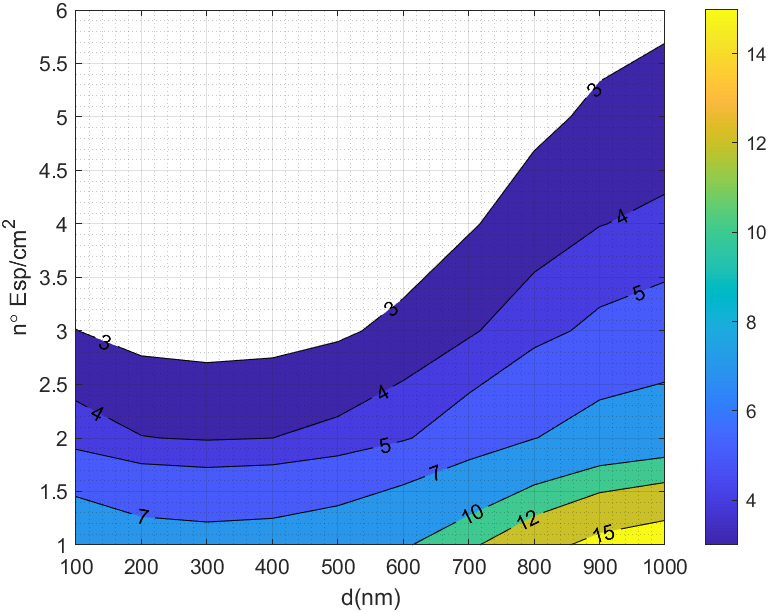
\includegraphics[width=0.8\columnwidth]{SiGe}
								\label{fig:SiSiO2Ge_rel}%Pn_SiCSiO2Ge
						\end{figure}
						\end{minipage}\hfill \vfill
						%%%%%%%%%%%%%%%%%%%%%%%%%
						\begin{minipage}[l]{.1\columnwidth}
							\begin{turn}{90}
							\begin{minipage}[t]{80pt}
								\begin{block}{\centering Rango completo}
								\end{block}
							\end{minipage}
							\end{turn}
					\end{minipage}\hfill
					\begin{minipage}[r]{.9\columnwidth}
						\begin{figure}[h]%
								\flushright
										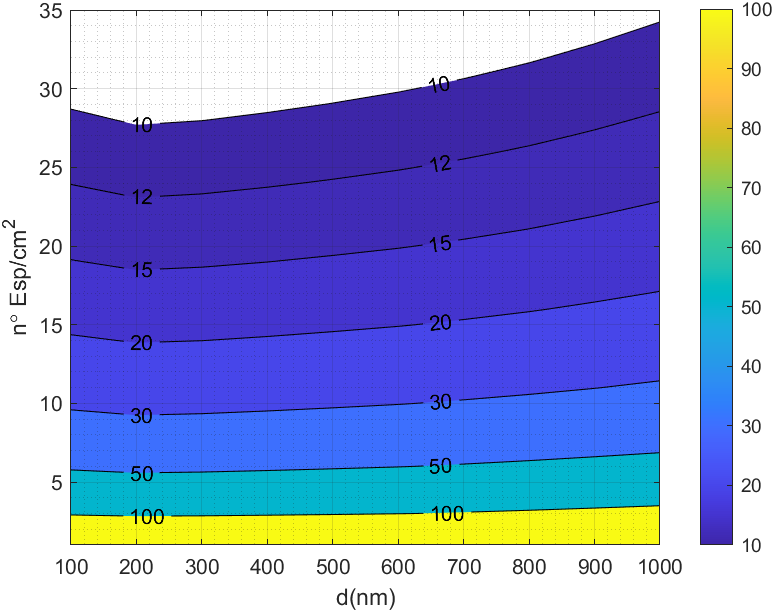
\includegraphics[width=0.8\columnwidth]{SiGe_full}
								\label{fig:SiSiO2Ge_relfull}%Pn_SiCSiO2Ge
						\end{figure}
						\end{minipage}
						\hfill \vfill
						%%%%%%%%%%%%%%%%%%%%%%%%%%%%%%%%%%%%%%%%%%%%%%%%%%%%%%%%%%%%%5
				\column{.5\textwidth}
					\vspace{-10pt}
						\begin{block}{\centering Con Rc}
							\end{block}
					\vspace{0pt}
					\begin{minipage}[c]{.9\columnwidth}
						\begin{figure}[h]%
								\centering
										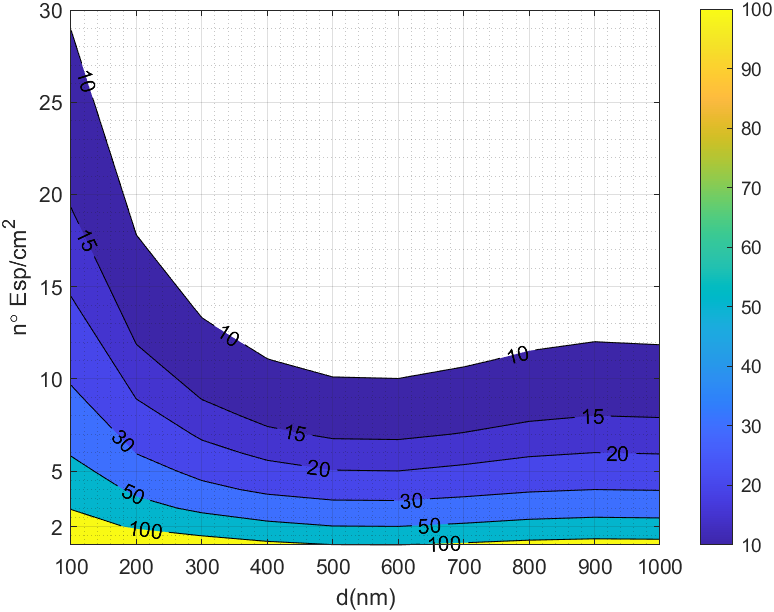
\includegraphics[width=0.81\columnwidth]{SiGe_Rc}%
								\label{fig:SiSiO2Ge_relRc}%
						\end{figure}
						\end{minipage}
						\hfill \vfill
						\begin{minipage}[c]{.9\columnwidth}
						\begin{figure}[h]%
								\centering
										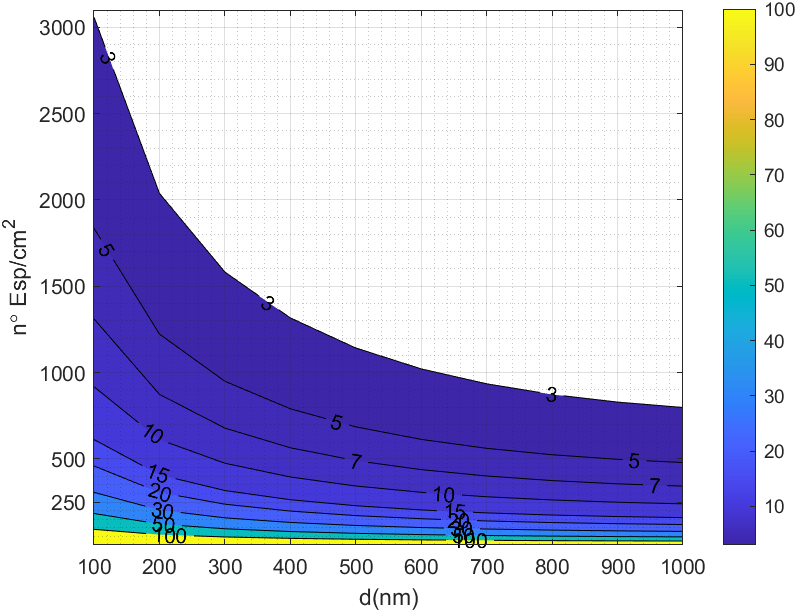
\includegraphics[width=0.81\columnwidth]{SiGe_Rc_full}
								\label{fig:SiSiO2Ge_relfullRc}%Pn_SiCSiO2Ge
						\end{figure}
						\end{minipage}
				\end{columns}		
		}
	\end{frame}
	
	\subsection{nTPV SS-SiO2-Ge}
		\begin{frame}{nTPV SS-SiO2-Ge}
	\only<1>{ %%%   CONDUCCION
			\frametitle{Conducción}
			\resCondPath
			\begin{figure}[h]%
				\centering
				\begin{subfigure}[b]{0.48\textwidth}\centering
					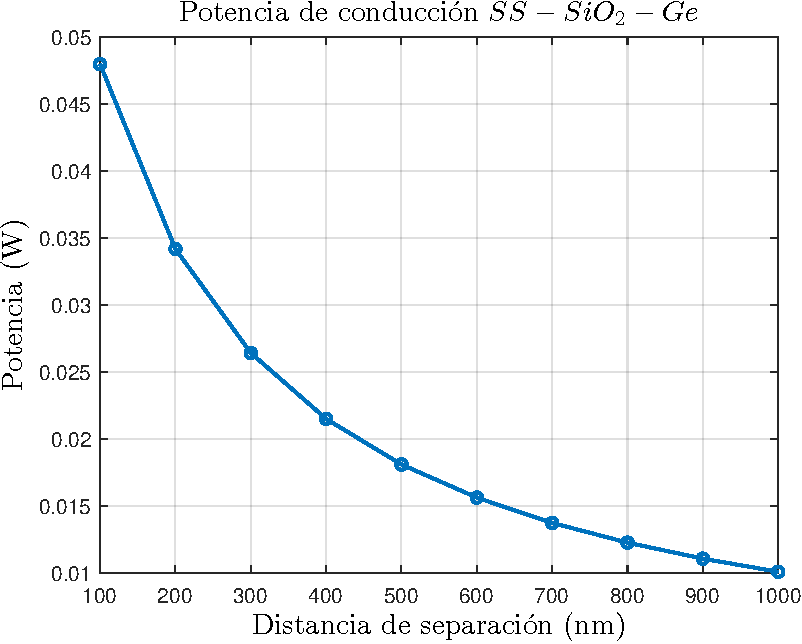
\includegraphics[width=0.8\textwidth]{Pn_SsSiO2Ge}%
				\end{subfigure}\hfill
				\begin{subfigure}[b]{0.48\textwidth}\centering
					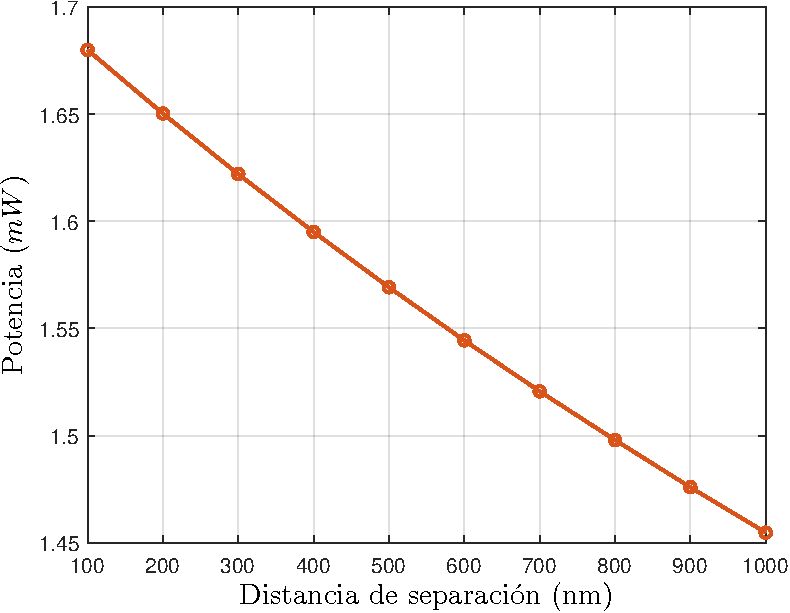
\includegraphics[width=.8\textwidth]{Prc_SsSiO2Ge_Emp}%
				\end{subfigure}\hfill
				\begin{subfigure}[b]{0.48\textwidth}\centering
					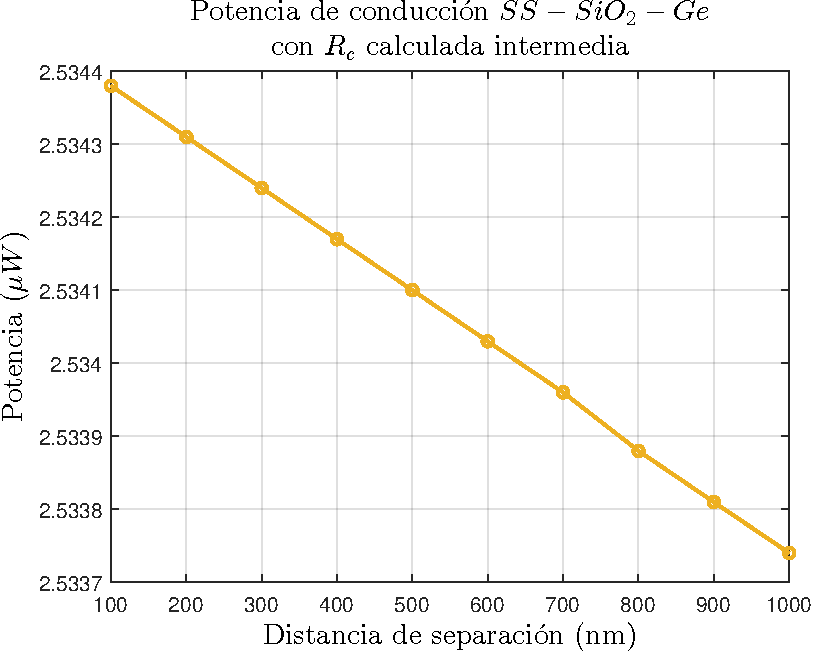
\includegraphics[width=.8\textwidth]{Prc_SsSiO2Ge_Inter}%
				\end{subfigure}\hfill
				\begin{subfigure}[b]{0.48\textwidth}\centering
					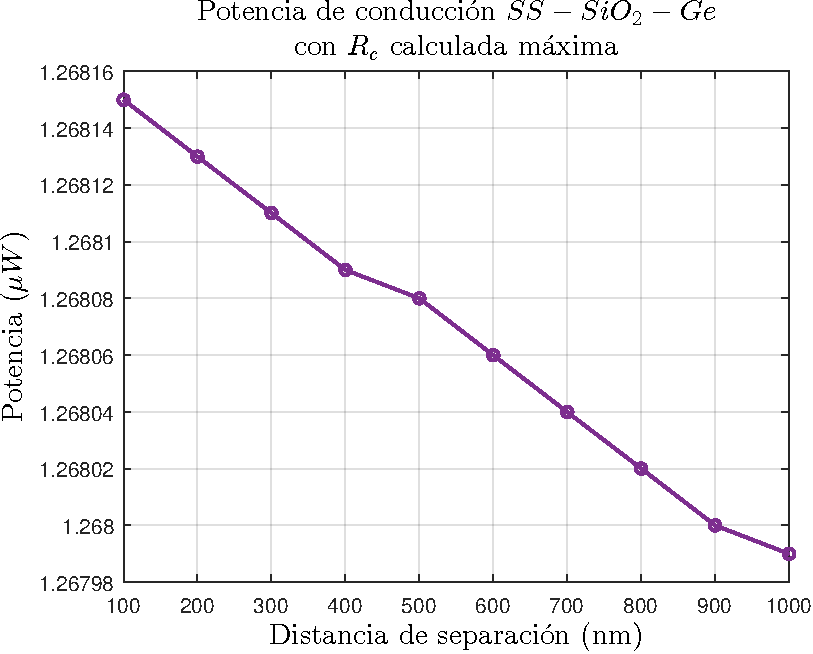
\includegraphics[width=.8\textwidth]{Prc_SsSiO2Ge_Max}%
				\end{subfigure}
			\label{}%
			\end{figure}					
		}
		%%%  RADIACION
		\only<2>{
			\frametitle{Radiación}
			\resRadPath
			\begin{columns}
			%%
				\column{.5\textwidth}
					%\vspace{-10pt}
						\begin{block}{\centering Por longitud de onda}
						\end{block}
					\vspace{15pt}
						\begin{figure}[h]%
								\centering
										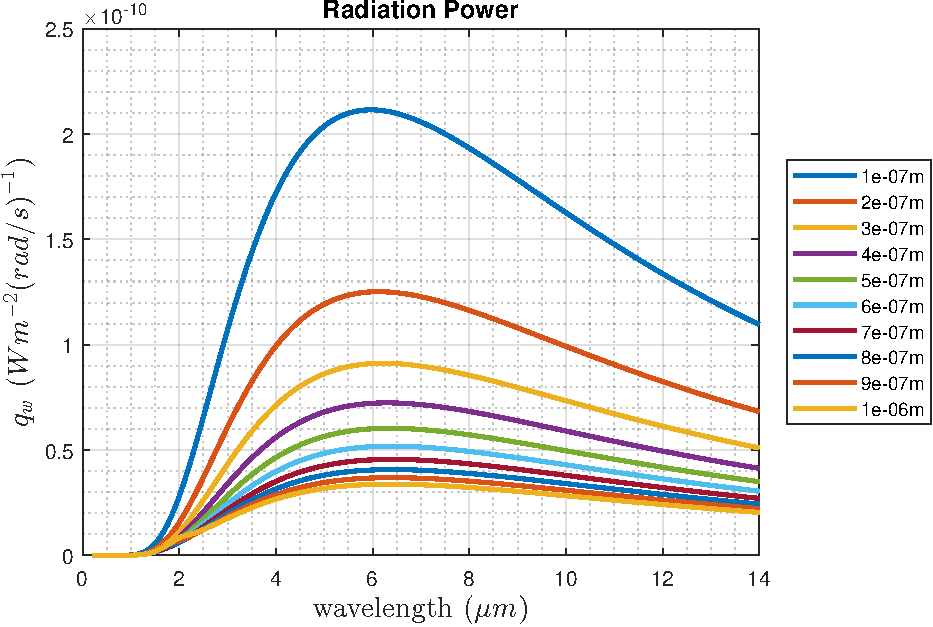
\includegraphics[width=\columnwidth]{SsGe}
								\label{fig:SsSiO2Ge_rad}%Pn_SiCSiO2Ge
						\end{figure}
						\vfill
						%%
				\column{.5\textwidth}
					\vspace{-10pt}
						\begin{block}{\centering En el rango de $E>0.7eV$}
							\end{block}
					\vspace{10pt}
						\begin{figure}[h]%
								\centering
										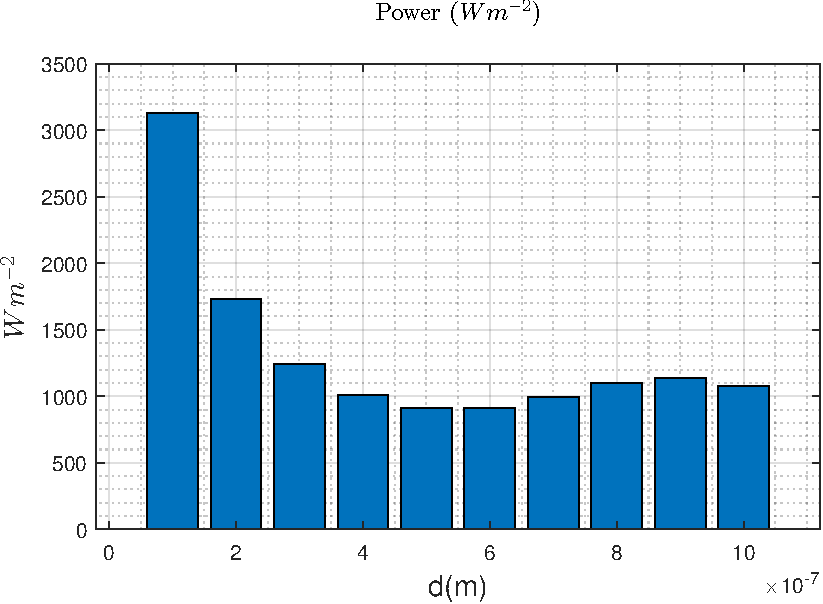
\includegraphics[width=\columnwidth]{p_Eg_SsGe}%
								\label{fig:SsSiO2Ge_radInt}%
						\end{figure}
						\vfill
				\end{columns}		
		}	
		\only<3>{
			\frametitle{Densidades de nano-espaciadores para $E>0.7eV$}
			\resRelPath
			\vspace{-5pt}
			\begin{figure}[h]%
				\centering
				\begin{subfigure}[b]{0.48\textwidth}\centering
					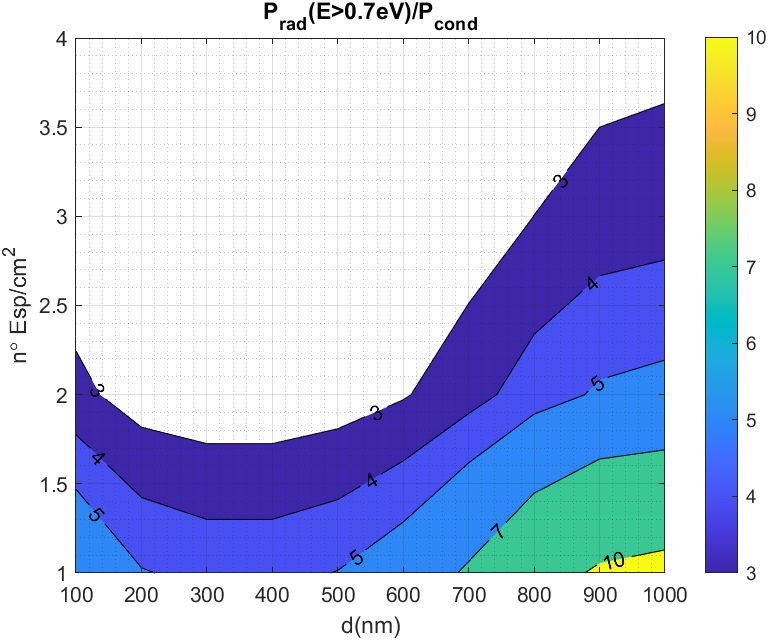
\includegraphics[width=0.8\textwidth]{SS}%
				\end{subfigure}\hfill
				\begin{subfigure}[b]{0.48\textwidth}\centering
					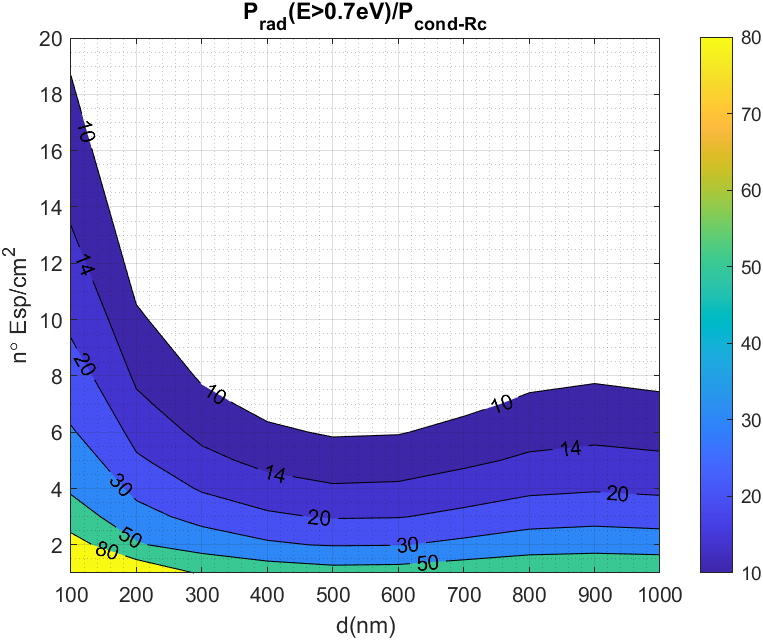
\includegraphics[width=.8\textwidth]{SS_Rc_empirico}%
				\end{subfigure}\hfill
				\begin{subfigure}[b]{0.48\textwidth}\centering
					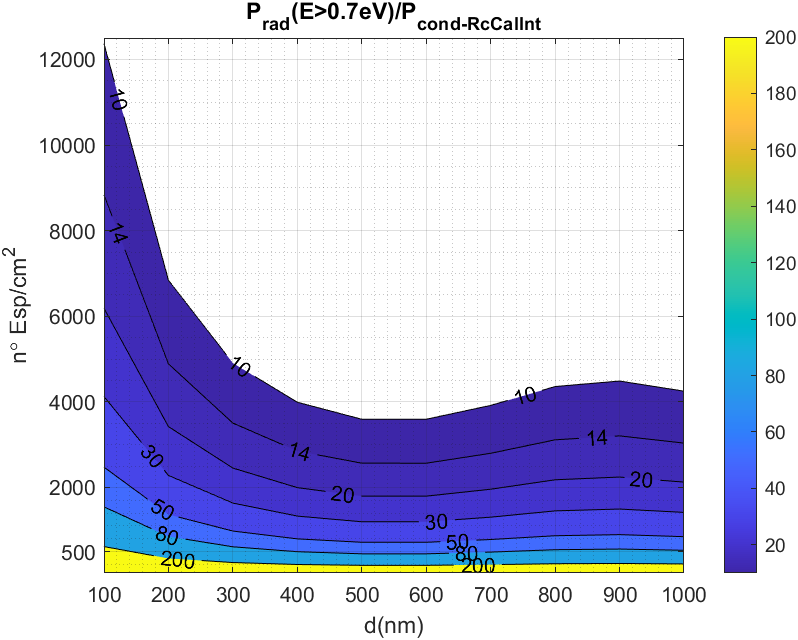
\includegraphics[width=.8\textwidth]{SS_Rc_Intermedio}%
				\end{subfigure}\hfill
				\begin{subfigure}[b]{0.48\textwidth}\centering
					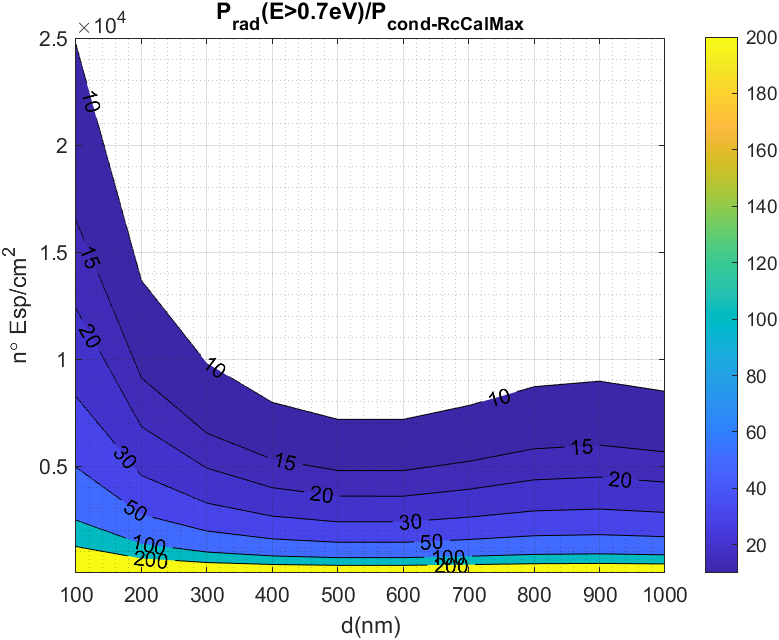
\includegraphics[width=.8\textwidth]{SS_Rc}%
				\end{subfigure}
			\label{SsSiO2Ge_rel}%
			\end{figure}	
		}
	\end{frame}
	
	\subsection{nTPV SiC-SiO2-Ge}
	\begin{frame}{nTPV SiC-SiO2-Ge}
		\only<1>{ %%%   CONDUCCION
			\frametitle{Conducción}
			\resCondPath
			\begin{columns}
			%%
				\column{.5\textwidth}
					%\vspace{-10pt}
						\begin{block}{\centering Sin Rc}
						\end{block}
					\vspace{15pt}
						\begin{figure}[h]%
								\centering
										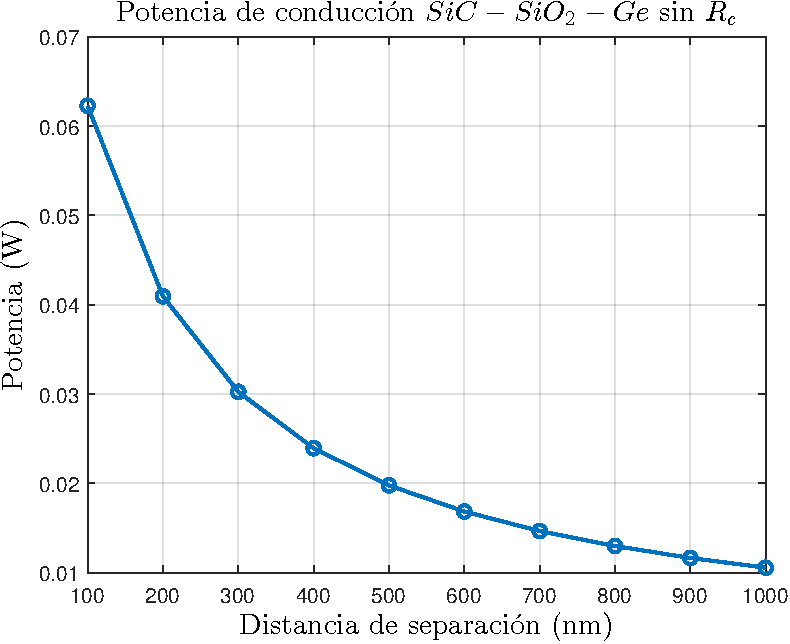
\includegraphics[width=\columnwidth]{Pn_SiCSiO2Ge}
								\label{fig:SiCSiO2Ge_cond}%Pn_SiCSiO2Ge
						\end{figure}
						\vfill
						%%
				\column{.5\textwidth}
					\vspace{-15pt}
						\begin{block}{\centering Con Rc}
							\end{block}
					\vspace{10pt}
						\begin{figure}[h]%
								\centering
										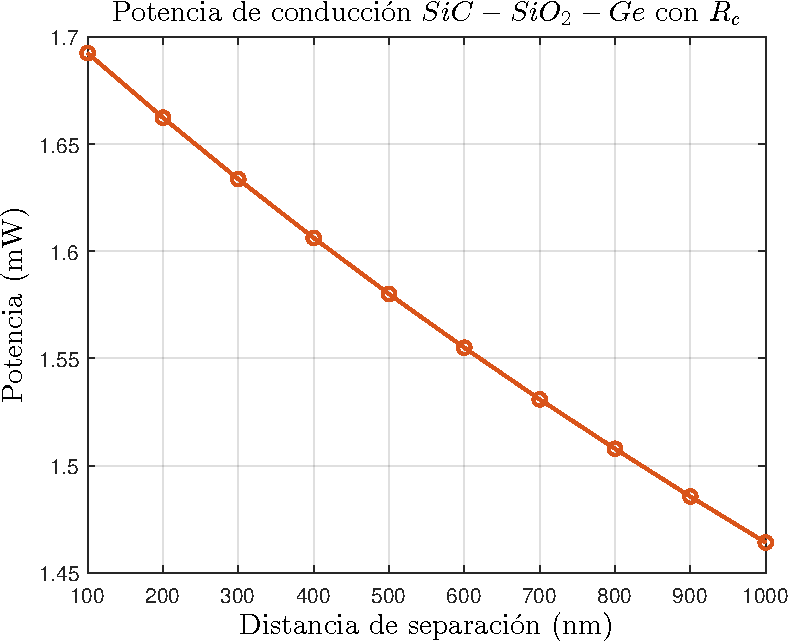
\includegraphics[width=\columnwidth]{Prc_SiCSiO2Ge}%
								\label{fig:SiCSiO2Ge_condRc}%
						\end{figure}
						\vfill
				\end{columns}							
		}
		%%%  RADIACION
		\only<2>{
			\frametitle{Radiación}
			\resRadPath
			\begin{columns}
			%%
				\column{.5\textwidth}
					%\vspace{-10pt}
						\begin{block}{\centering Por longitud de onda}
						\end{block}
					\vspace{15pt}
						\begin{figure}[h]%
								\centering
										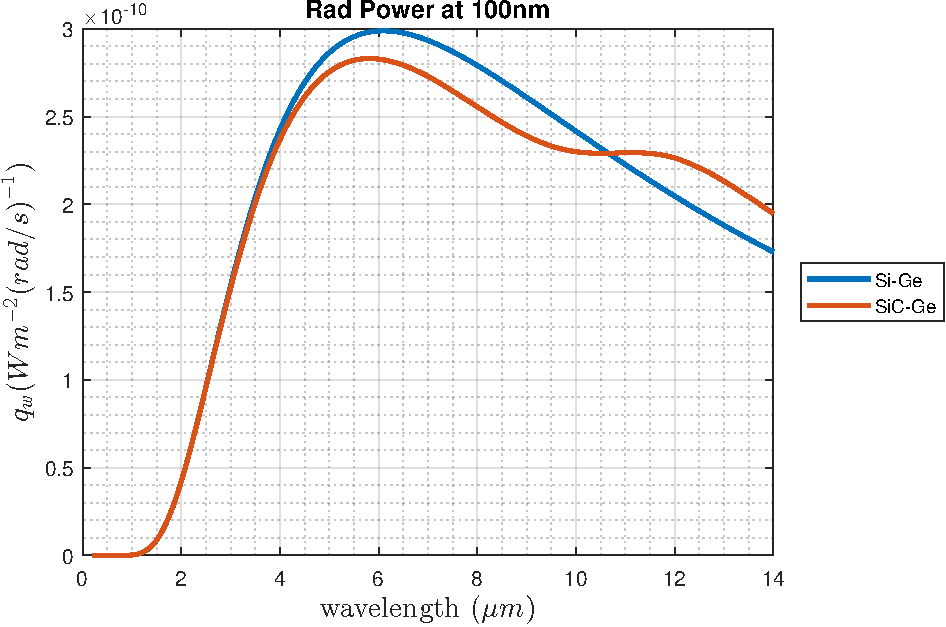
\includegraphics[width=\columnwidth]{SiCvsSi_rad}
								\label{fig:SiCGevsSiGe_rad}%Pn_SiCSiO2Ge
						\end{figure}
						\vfill
						%%
				\column{.5\textwidth}
					\vspace{-10pt}
						\begin{block}{\centering En el rango de $E>0.7eV$}
							\end{block}
					\vspace{10pt}
						\begin{figure}[h]%
								\centering
										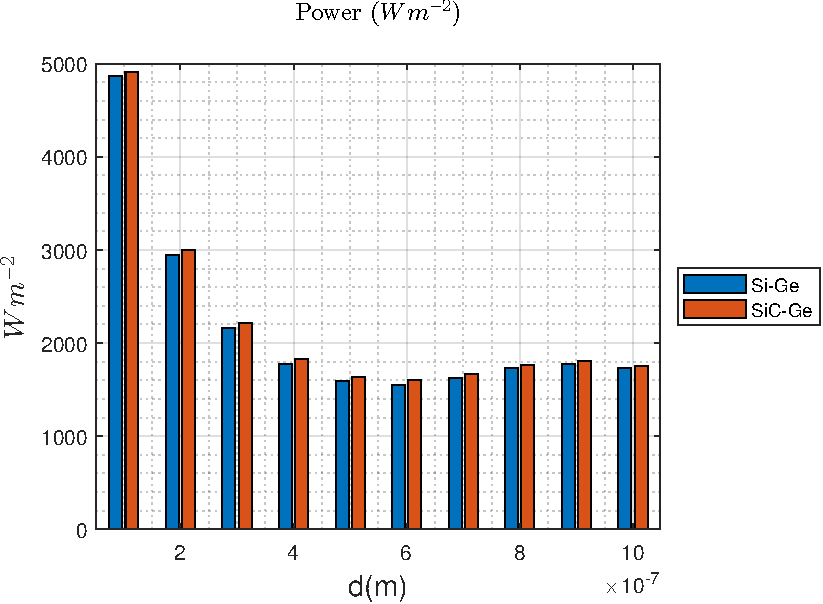
\includegraphics[width=\columnwidth]{SiCvsSi}%
								\label{fig:SiCGevsSiGe_radInt}%
						\end{figure}
						\vfill
				\end{columns}		
		}
				\only<3>{
			\frametitle{Densidades de nano-espaciadores ({\small $n^{\circ}esp/cm^2$}) y {\small $E>0.7eV$}}
			\resRelPath
			\begin{columns}
			%%
				\column{.5\textwidth}
					%\vspace{-1cm}
						\begin{block}{\centering Sin Rc}
						\end{block}
					\vspace{10pt}
						\begin{figure}[h]%
								\centering
										\includegraphics[width=\columnwidth]{SiC_Ge}
								\label{fig:SiCSiO2Ge_rel}%Pn_SiCSiO2Ge
						\end{figure}
						\vfill
						%%
				\column{.5\textwidth}
					\vspace{-12pt}
						\begin{block}{\centering Con Rc}
							\end{block}
					\vspace{10pt}
						\begin{figure}[h]%
								\centering
										\includegraphics[width=\columnwidth]{SiC_Rc}%
								\label{fig:SiCSiO2Ge_relRc}%
						\end{figure}
						\vfill
				\end{columns}		
		}
		\only<4>{
		\frametitle{Frecuencia de resonancia ($\omega_{res}$)}
			\resRadPath
		\begin{figure}[h]
			\centering
				\includegraphics[width=.8\textwidth]{SiCSiC.pdf}
			\label{fig:SiCSiC}
		\end{figure}
		
		}
	\end{frame}
	
	\subsection{Densidad de carga}
	\begin{frame}{Densidad de carga}
	\vspace{-20pt}
	{\footnotesize
	Densidad de nano-espaciadores ($n^{\circ}esp/cm^2$) para soportar cargas aplicadas sobre los nano-espaciadores. Se consideran viables si para la densidad obtenida la relación de potencias es mayor a un orden de magnitud.
	}
	\vspace{10pt}
	\begin{block}{Carga de acero inoxidable ($\rho = 8\ gr/cm^3$) de $0.5\ cm^3$}
		Para una carga de $\sim 0.04 \ N \ \Longrightarrow \ 3 \ n^{\circ}esp/cm^2$.\\ Viable para nTPVs con $R_cEmp$.
	\end{block}
		\begin{block}{Carga de acero inoxidable de $0.5\ cm^3$ y una atmósfera de presión}
		La carga se dispara a $10.17 \ N \ \Longrightarrow \ 673 \ n^{\circ}esp/cm^2$.\\ Viable para nTPVs con $R_cCal$.
	\end{block}

	\end{frame}
	
%% CONCLUSIONES
	\section{Conclusiones}
	\begin{frame}{Conclusiones}
	\setbeamertemplate{itemize items}[triangle]
	\only<1-3>{
	
		\begin{itemize}
			\item La porosidad de los nano-espaciadores no es tan importante.
			\item<2-3> El uso de células de menor banda energética es indispensable para obtener mayores potencias.
			\item<3> Las resistencias de contacto es el factor más importante, sí es el de mayor relevancia.
			
		\end{itemize}
	}
	\only<4-7>{
	\framesubtitle{Importancia de la resistencia de contacto}
		\setbeamertemplate{itemize items}[circle]
			\begin{itemize}
				\item<4-7> Disminución de las pérdidas por conducción.
				\item<5-7> Solo las nTPVs con $R_c$ pueden soportar cargas (orden de los $10^{-3} m^2 K/W$).
				\item<6-7> Diferentes materiales de nano-espaciadores ($R_c>4\cdot 10^{-6} m^2 K/W$).
				\item<7> El material de emisor afecta principalmente a la radiación.
			\end{itemize}			
	}	
	\end{frame}
	\begin{frame}{Estudios a futuro}
		\begin{itemize}
			\item<1-> Estudiar en detalle la resistencia de contacto.
			\item<2-> Diferentes materiales de nano-espaciadores
			\item<3-> Sistemas multi-capa en emisor y uso de células multi-uniones.
			\item<4-> Diseñar una app para cálculos de rad. de campo cercano de sistemas multi-capa.			
		\end{itemize}
	\end{frame}

%% FINAL
	\miniframesoff
	\section{ }
	\begin{frame}{Bibliografía}
        \bibliographystyle{apalike}
				\tiny
        \bibliography{bibliografia/bibliografia}		
	\end{frame}
	\begin{frame}{}
		\begin{block}{\Huge \centering¡Gracias por su atención!}
		\end{block}
	\end{frame}
\end{document}
